\documentclass[10pt]{article}
\usepackage{amsmath}
\usepackage{listings}
\usepackage{graphicx}
\usepackage{float}
\usepackage{tabularx}
\graphicspath{ {./images/} }
\begin{document}
{\centering
    CSU44061 Machine Learning - Week 6
    \par
    Samuel Petit - 17333946
    \par
    Dataset \# id:8--80--16 
    \par
}
\section*{Question i}
Code for all questions provided in the appendix.

\subsection*{Part a}
Let's start with going through what we need to train these models, first we need to generate our dataset.
Using the linspace method over the range -1 to 1 with 3 number of data points,
we generate our X points. I then hardcoded the Y values. In order to work
with the single feature, I reshape it thanks to panda's methods and we
are ready to use this data with sklearn models.

\begin{lstlisting}[language=Python]  
    m = 3
    Xtrain = np.linspace(-1.0, 1.0, num=m)
    ytrain = np.sign(np.array([0, 1, 0]))
    Xtrain = Xtrain.reshape(-1, 1)  
\end{lstlisting}

The gaussian kernel used is the same as previously used in lectures so I
won't spend too much time explaining it:

\begin{lstlisting}
def gaussian_kernel(distances):
    weights = np.exp(-V * (distances ** 2))
    return weights/np.sum(weights)
\end{lstlisting}

Note the use of V in that method. That is a global variable set within the
code such as to be able to change the V value of that method easily.

Finally, the last piece we need is the testing set of X values which, as stated
in the question is over the range [-3, 3]. I also use linspace to generate it:

\begin{lstlisting}
    Xtest = np.linspace(-3.0, 3.0, num=100).reshape(-1, 1)
\end{lstlisting}


Now, using all these and a range of $\gamma$ values, we can train a kNN model
which yeild the following predictions:


\begin{figure}[H]    
    \fbox{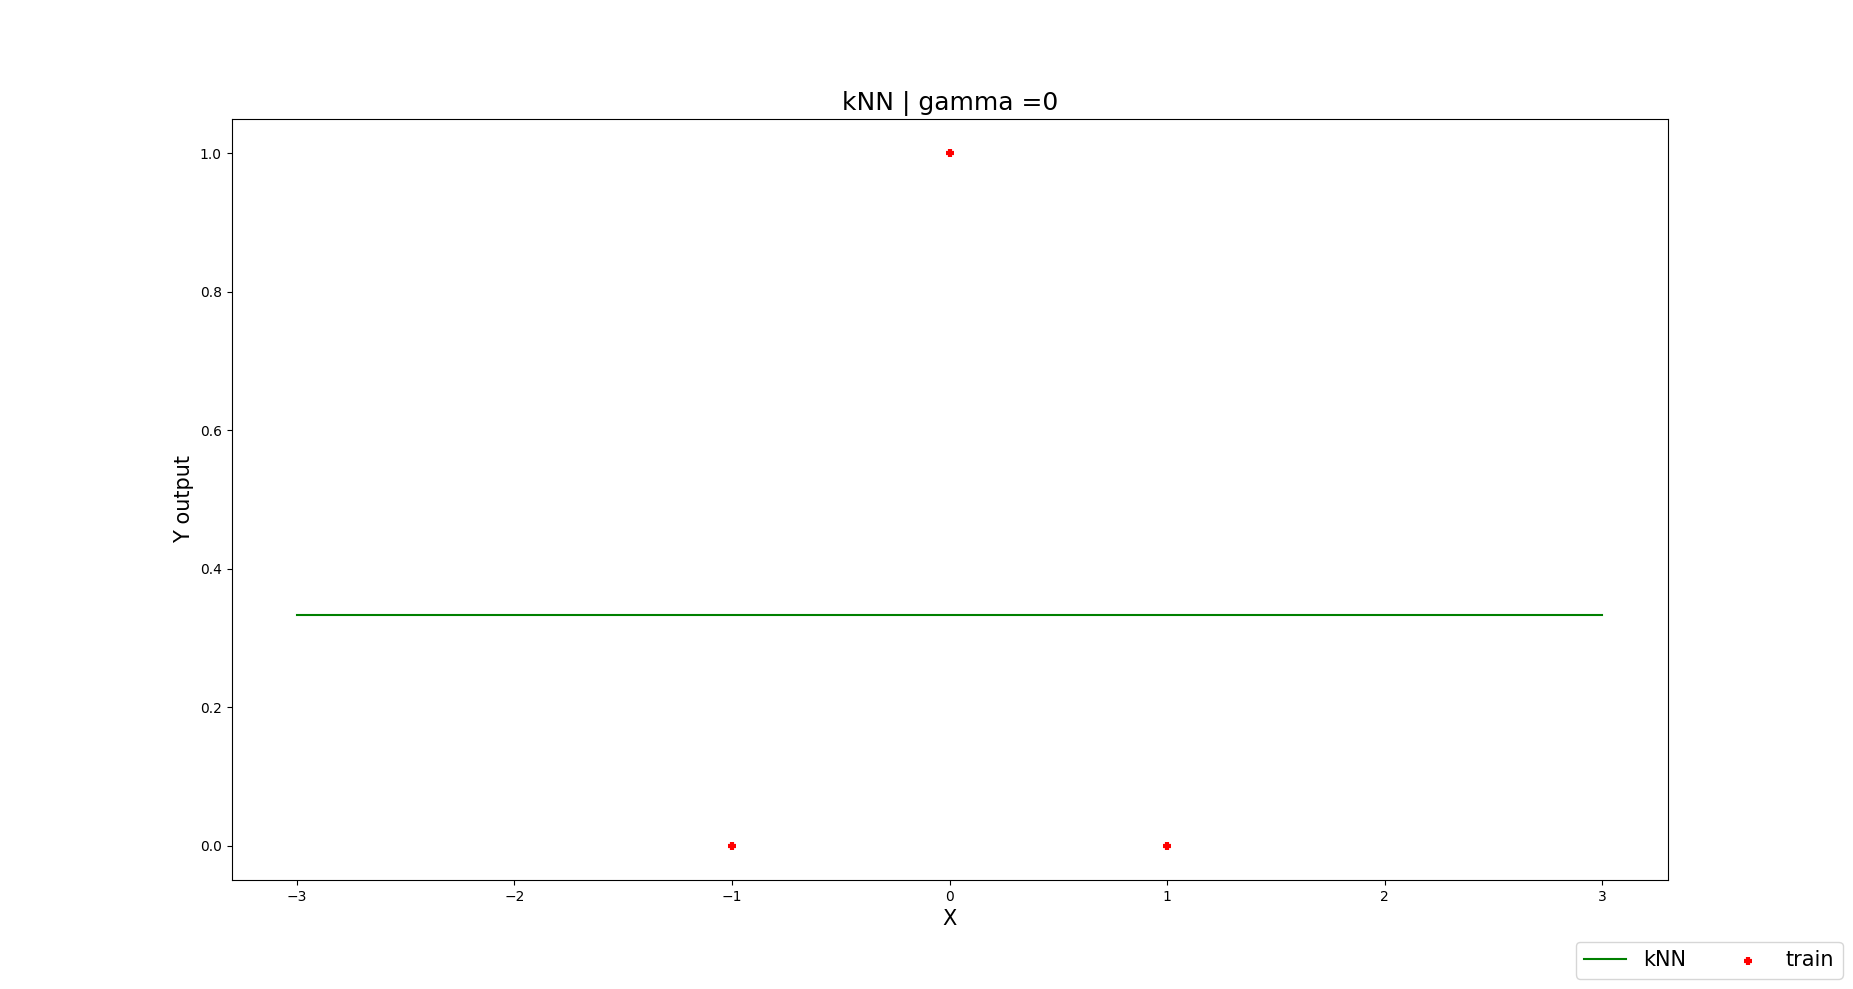
\includegraphics[scale=0.15]{knn_gamma_0.png}}   
    \fbox{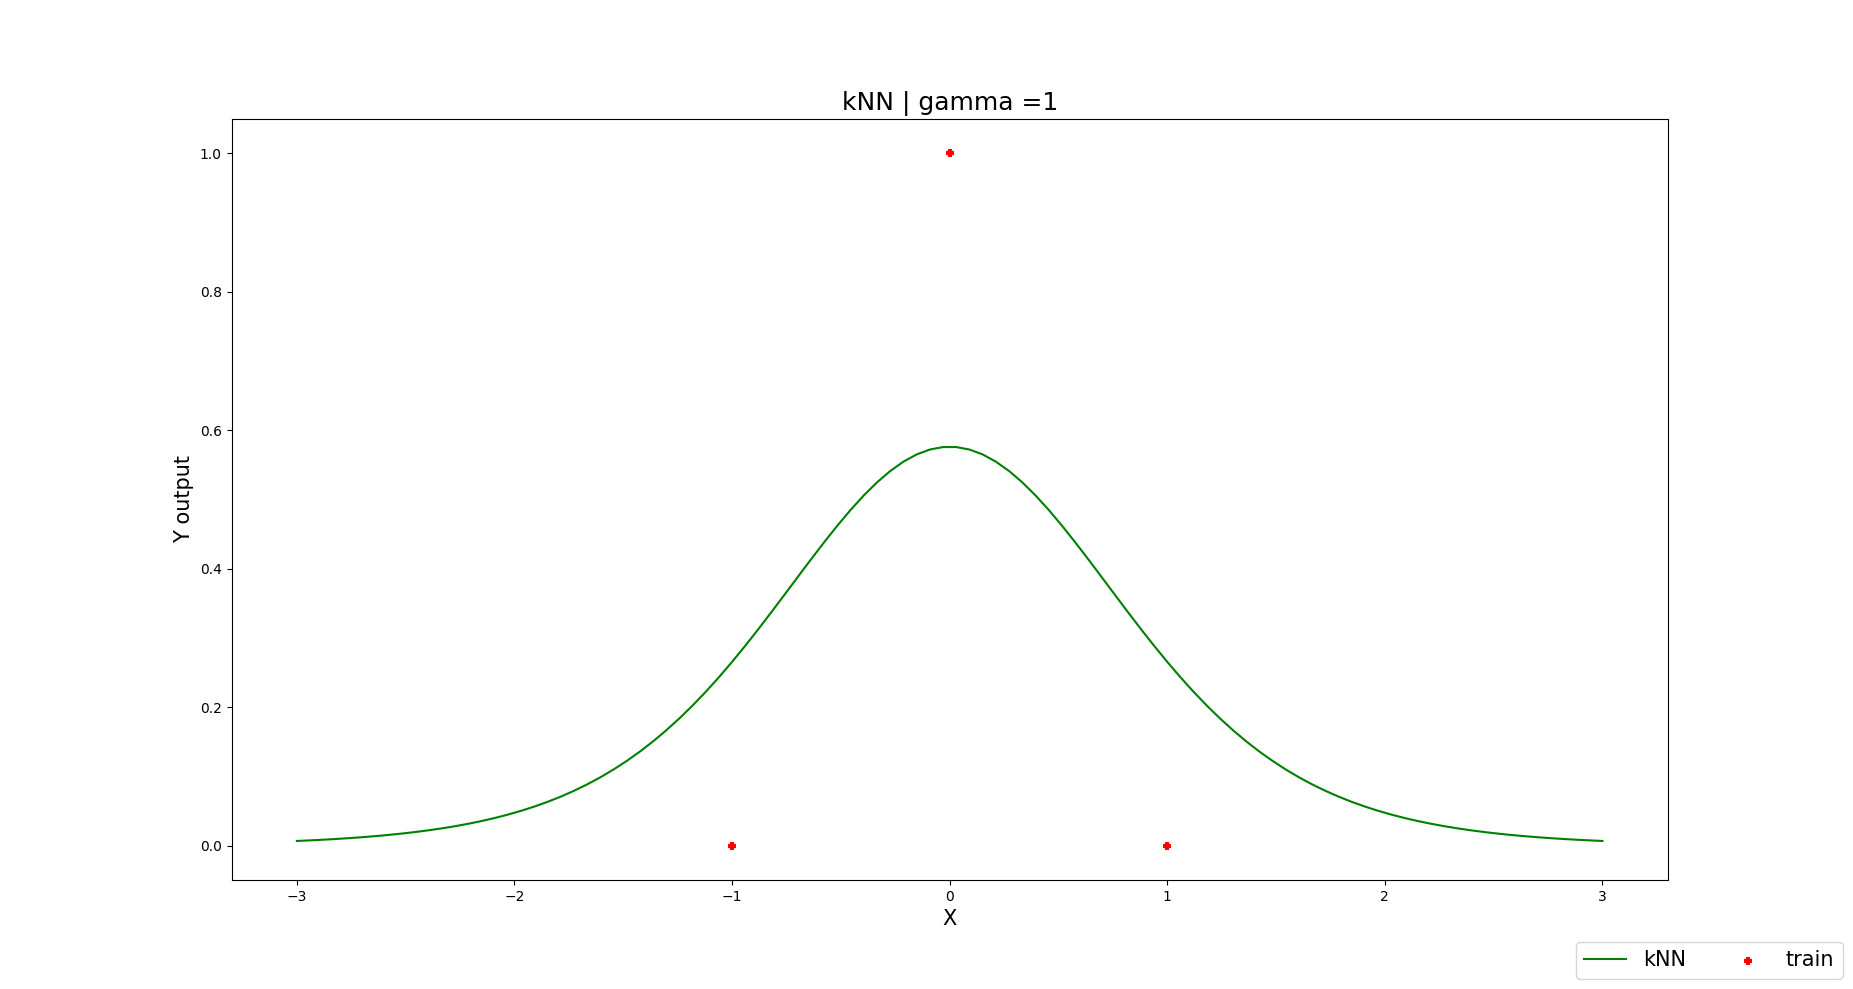
\includegraphics[scale=0.15]{knn_gamma_1.png}}   
    \fbox{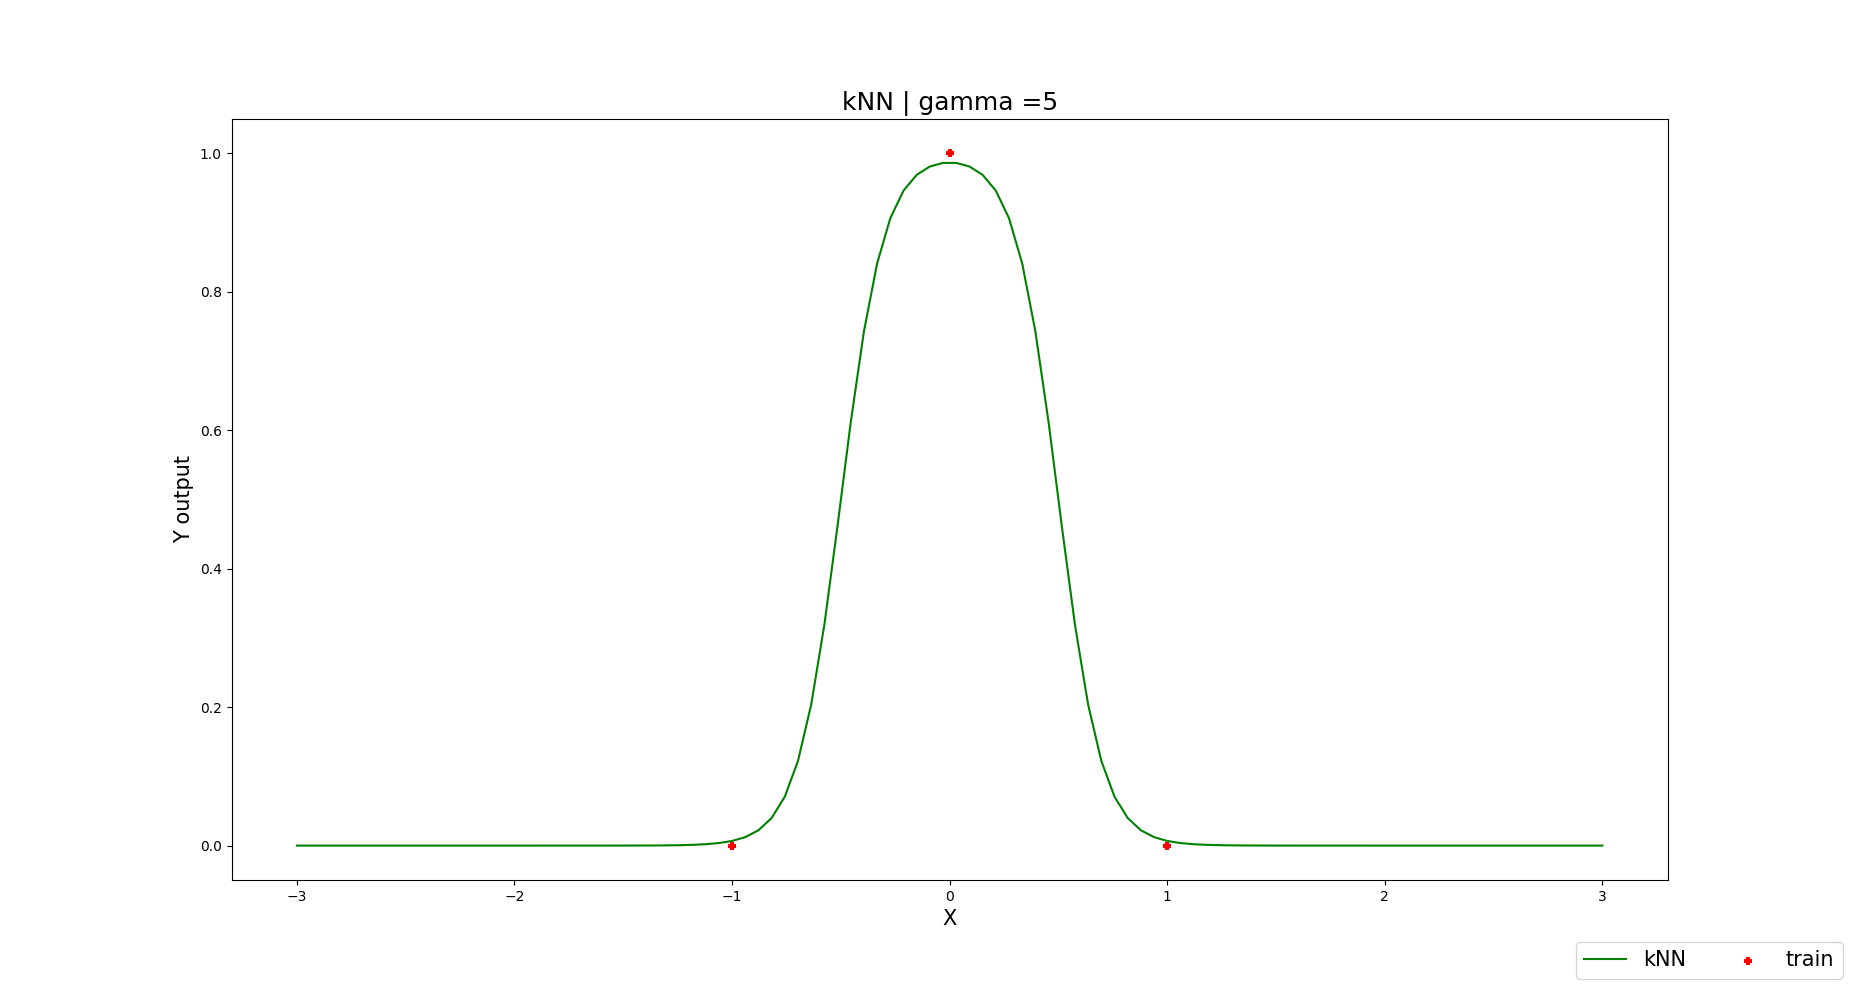
\includegraphics[scale=0.15]{knn_gamma_5.png}}
    \fbox{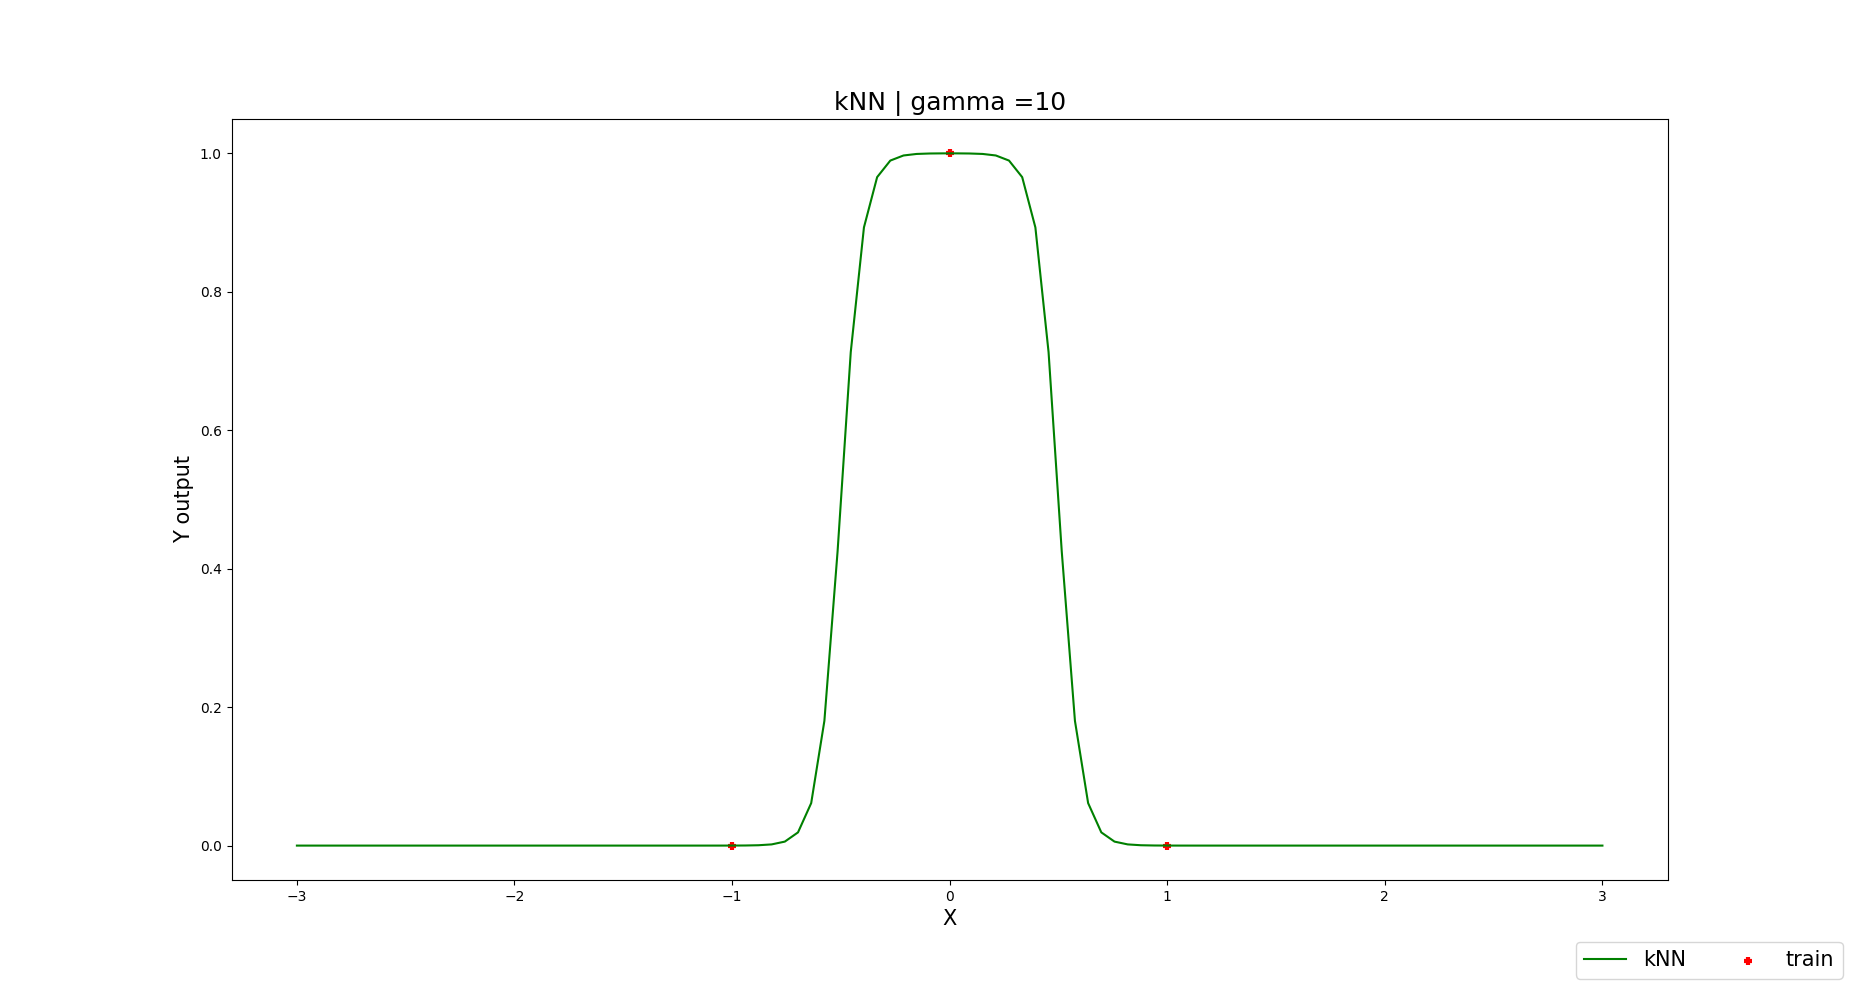
\includegraphics[scale=0.15]{knn_gamma_10.png}}
    \fbox{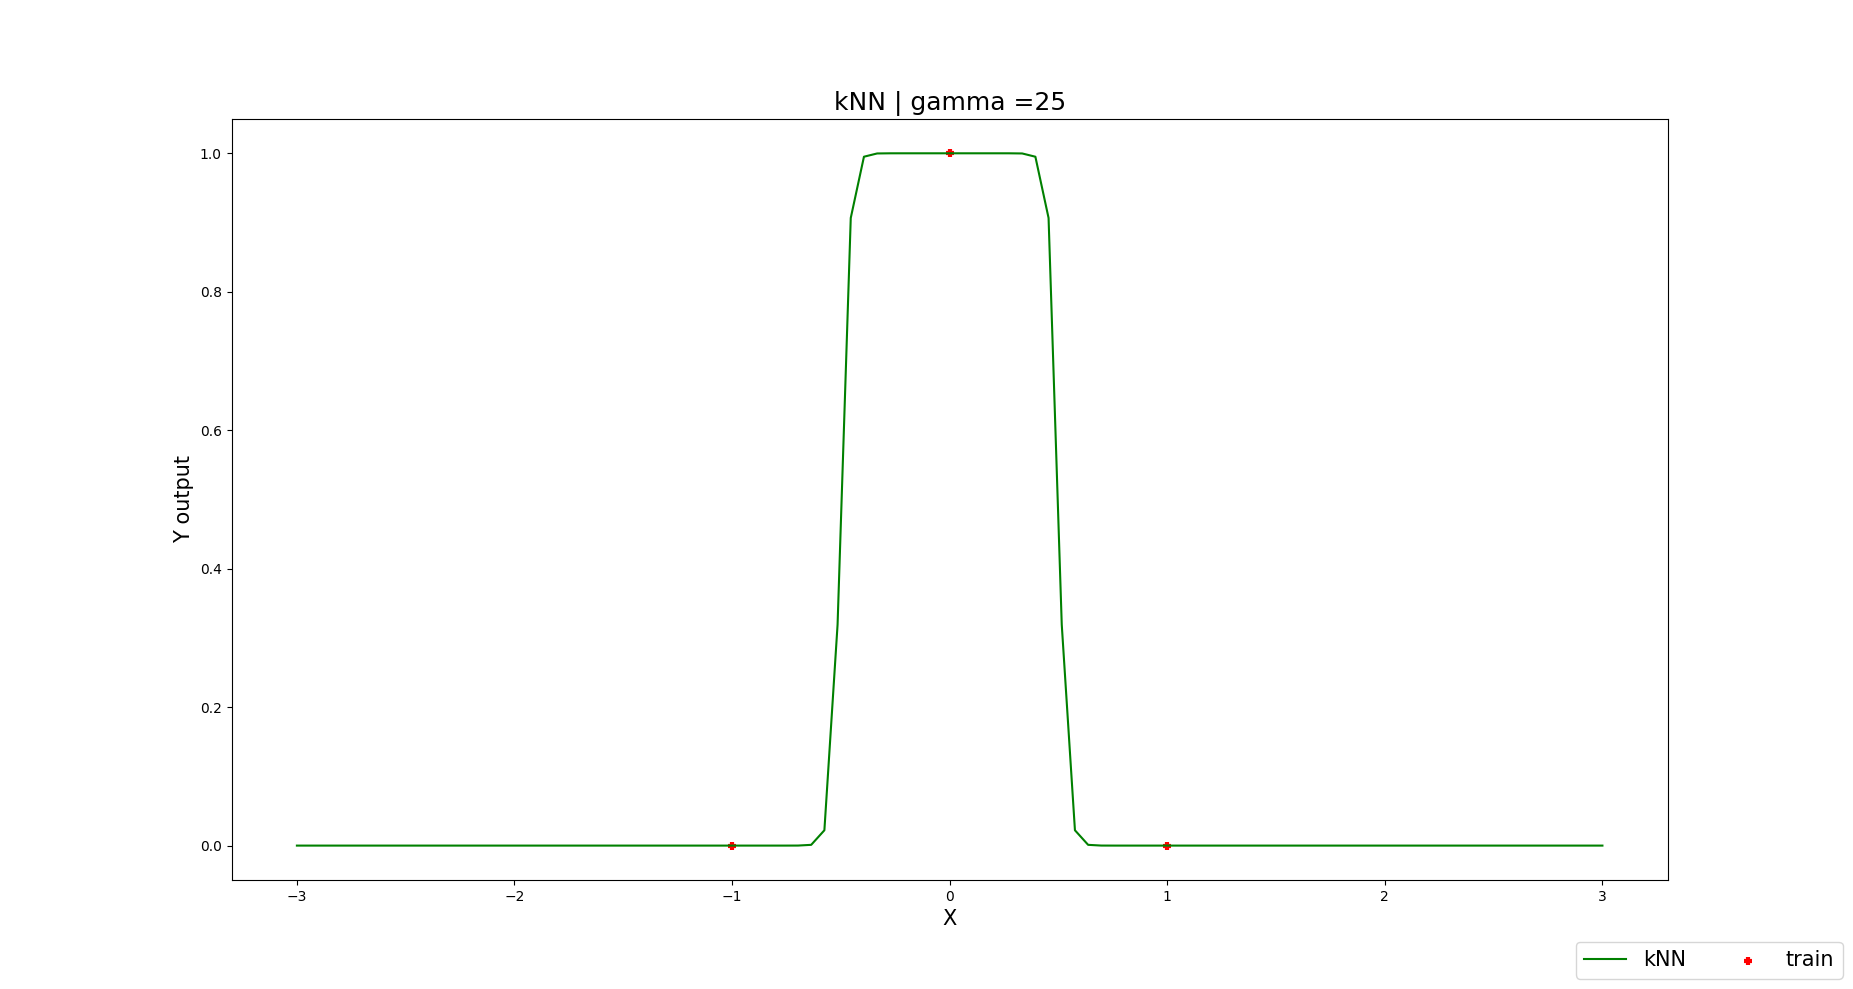
\includegraphics[scale=0.2]{knn_gamma_25.png}}
\end{figure}

\subsection*{Part b}
A kNN model makes predictions based on its closest neighbors, in a kNN regression it is the average of all
k neighbors. Here we use $ k = 3$ which is the entire dataset. However we also use a Gaussian function here which essentially means
our feature is mapped through the gaussian function which gives a form of distance estimation.

Given that 2 out of our 3 points are 0, we understand that value of $ \gamma = 0$ makes the gaussian function
not have an effect and thus our predictions take the form of a constant line that is closer to 0 than 1 on the y axis (the average of all
$k = 3$ neighbors).

We notice that the more we increase $\gamma$, the more our predictions tend to 1 for x values in the range [-0.5, 0.5] (roughly). We can clearly
see the impact of the gaussian function there, going from some form of a smooth quadratic shape to a more binary prediction model for high
values of $\gamma$, where it is predicting 0 most of the time, and 1 when x gets close to 0.

We've seen in class that as $\gamma$ grows, our value for $K(x^{i}, x)$ decreases much faster as the distance between $x^{i}$ and $x$ grows.
That is clearly noticeable as the plot for $\gamma = 25$ decreases much faster than say $\gamma = 1$ where we can see increases and decreases over
most of the range of x values.


\subsection*{Part c}
I won't go over explaining how the data was formatted and prepared again as that was covered in part a. Iterating over the provided range
of $ C = [0.1, 1, 1000] $ and $ \gamma = [0, 1, 5, 10, 25]$, we obtain the following graphs (grouped by their $\gamma$ value).
Note that the dual coef parameter is included within the title of each graph.


$\gamma$ = 0
\begin{figure}[H]    
    \fbox{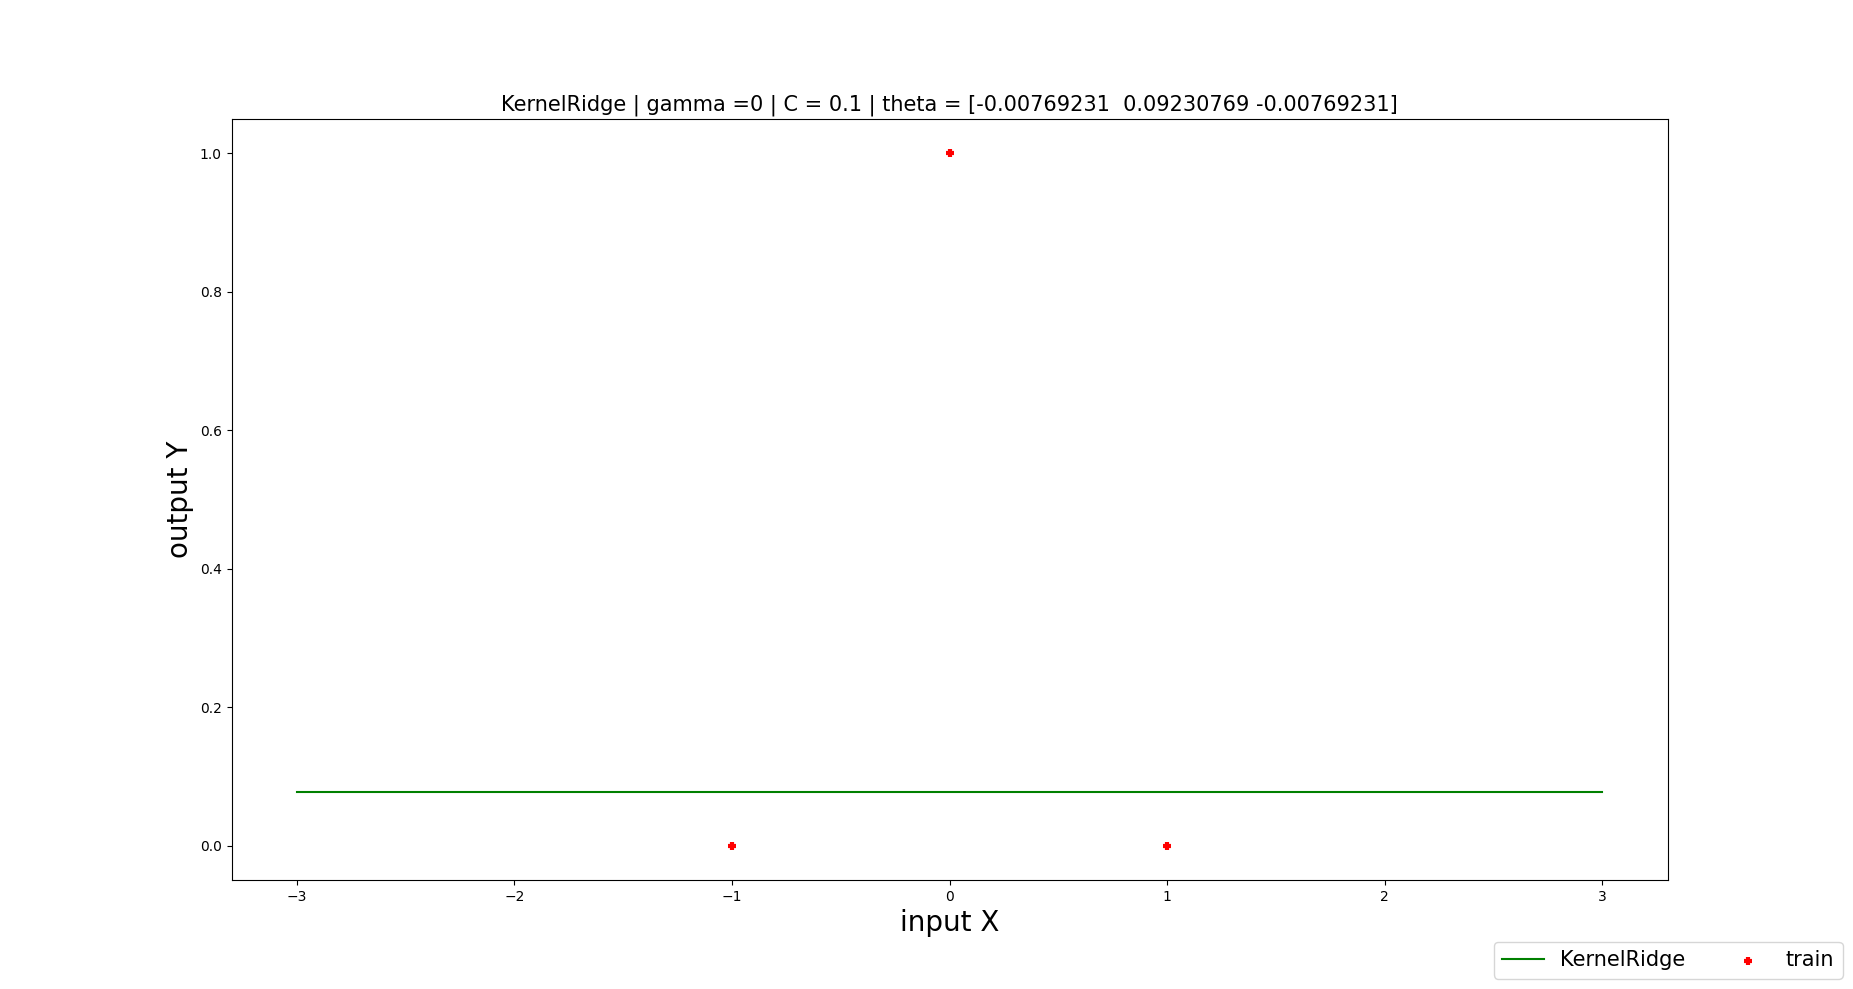
\includegraphics[scale=0.15]{kridge_gamma_0_c_01.png}}   
    \fbox{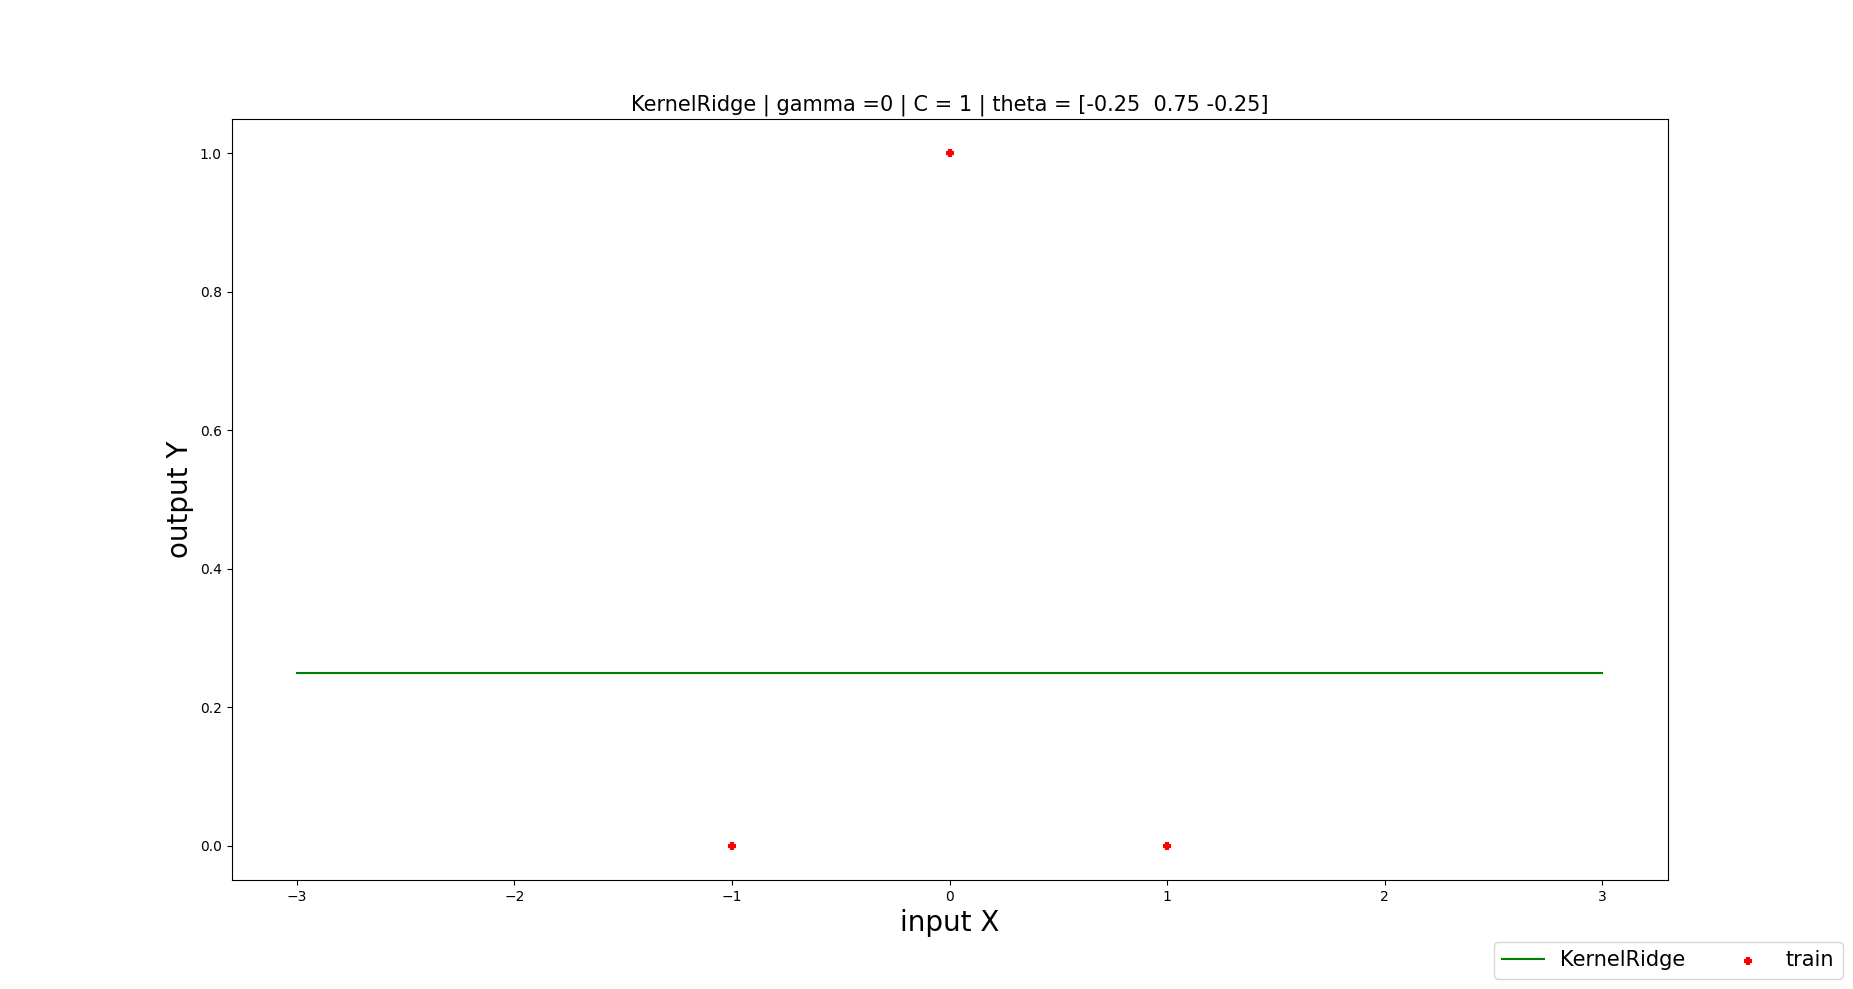
\includegraphics[scale=0.15]{kridge_gamma_0_c_1.png}}   
    \fbox{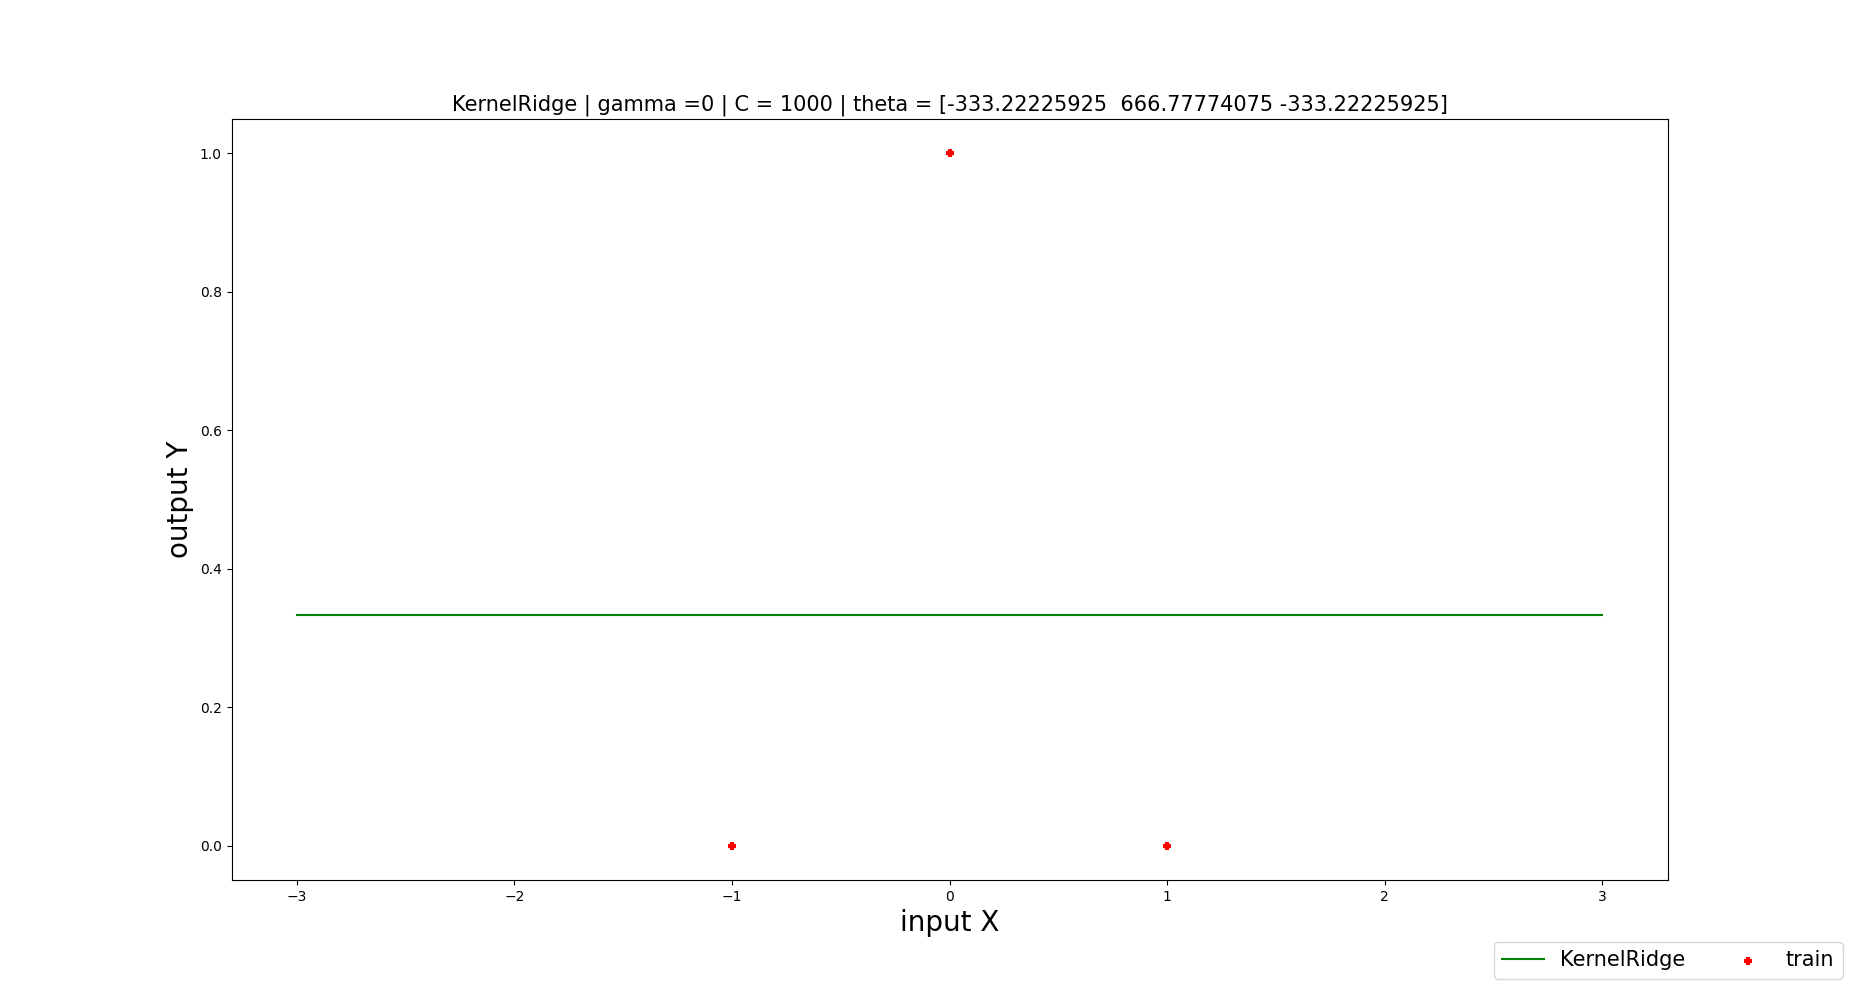
\includegraphics[scale=0.15]{kridge_gamma_0_c_1000.png}}
\end{figure}

\vspace{10mm} %5mm vertical space

$\gamma$ = 1
\begin{figure}[H]    
    \fbox{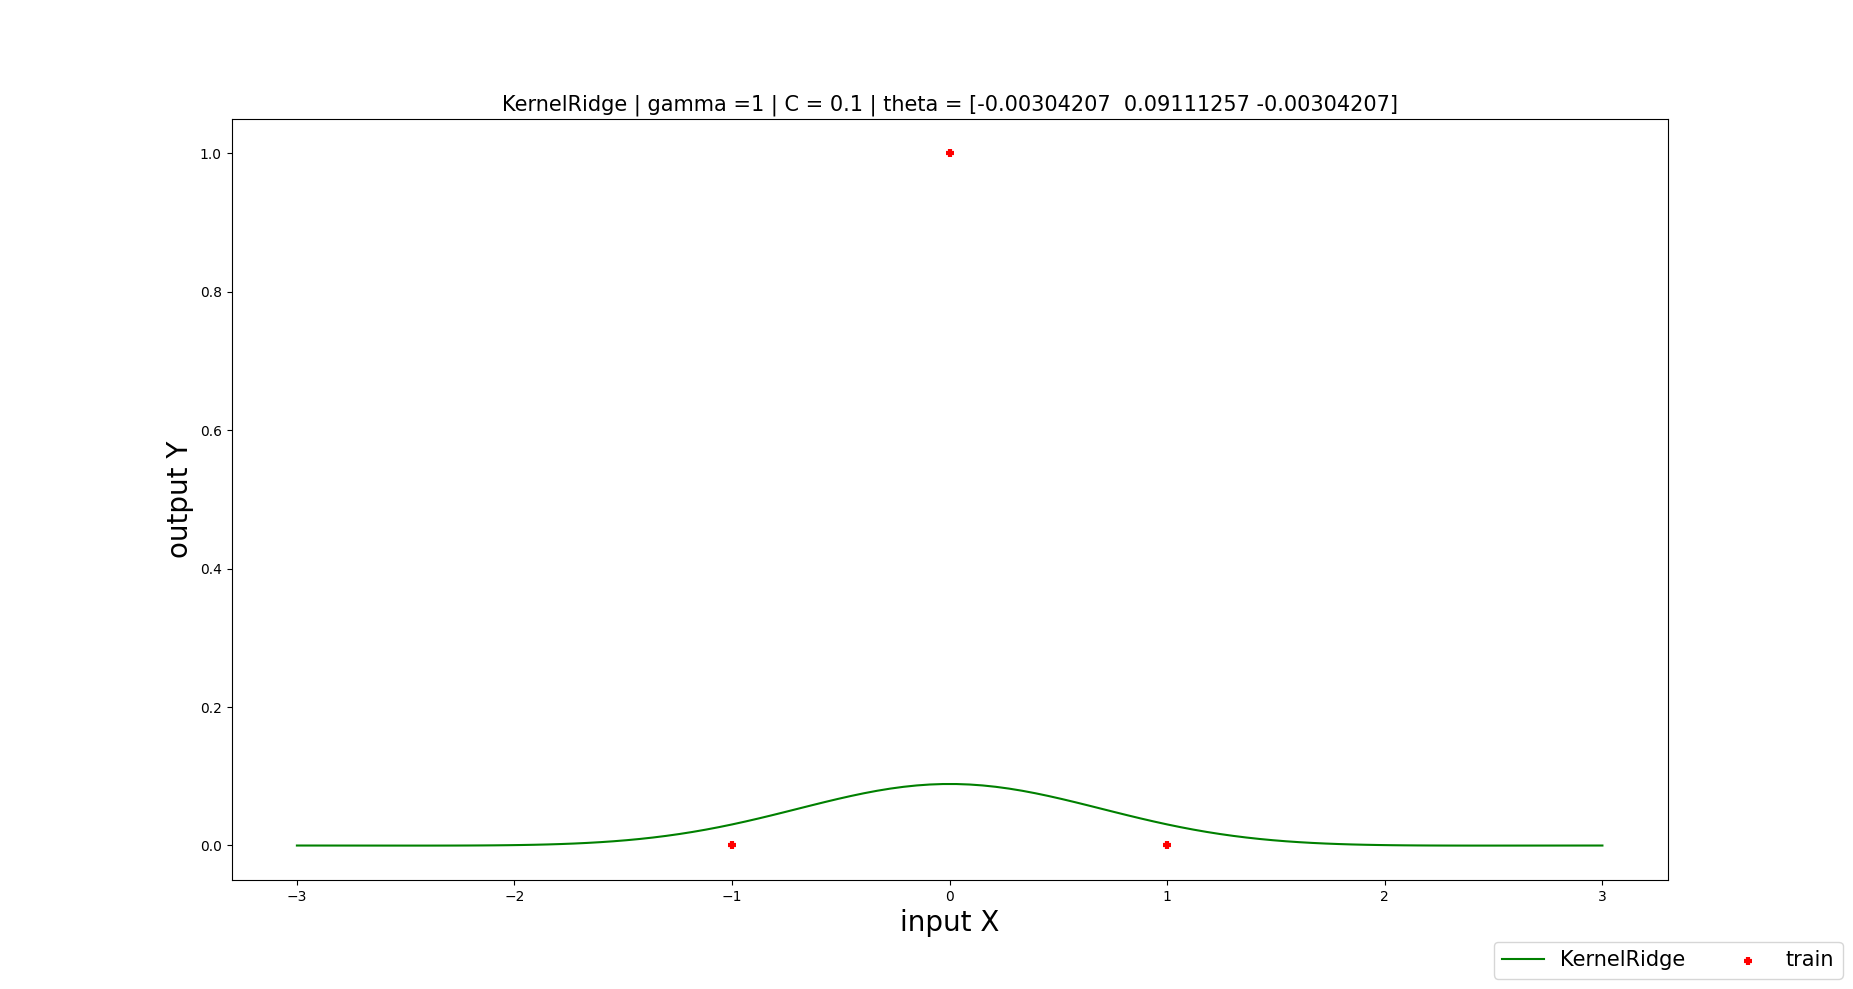
\includegraphics[scale=0.15]{kridge_gamma_1_c_01.png}}   
    \fbox{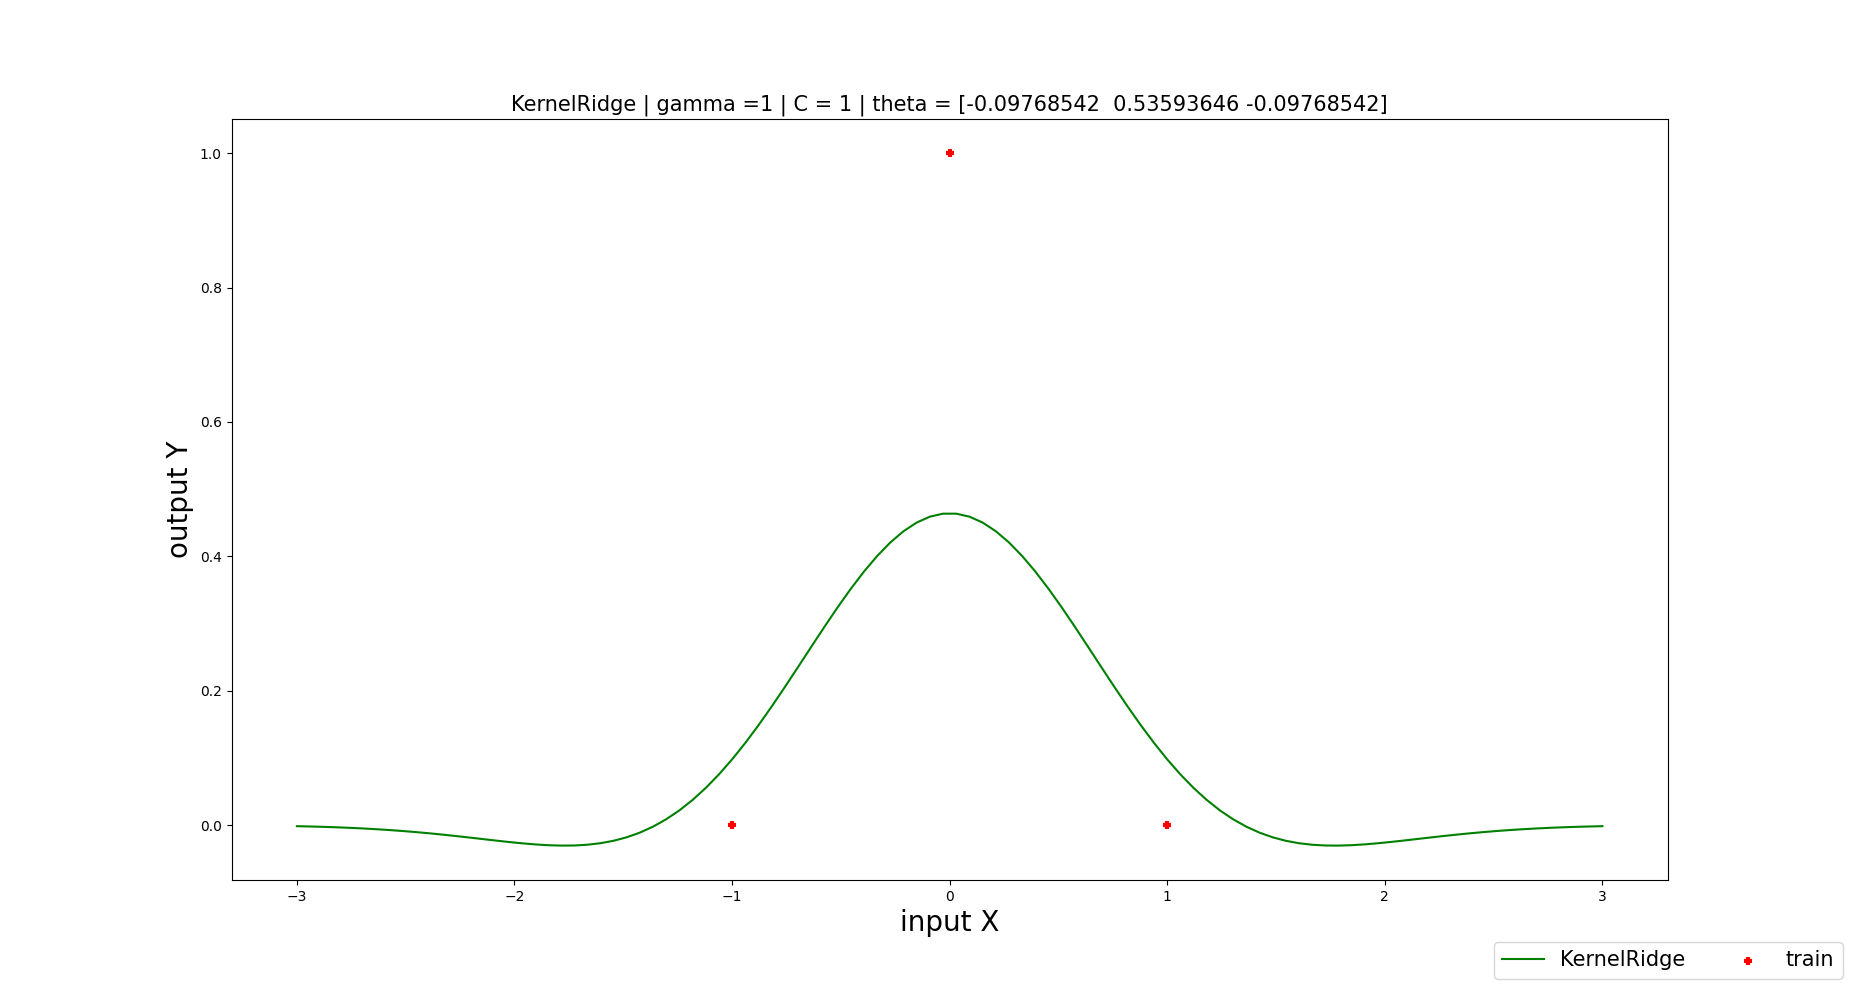
\includegraphics[scale=0.15]{kridge_gamma_1_c_1.png}}   
    \fbox{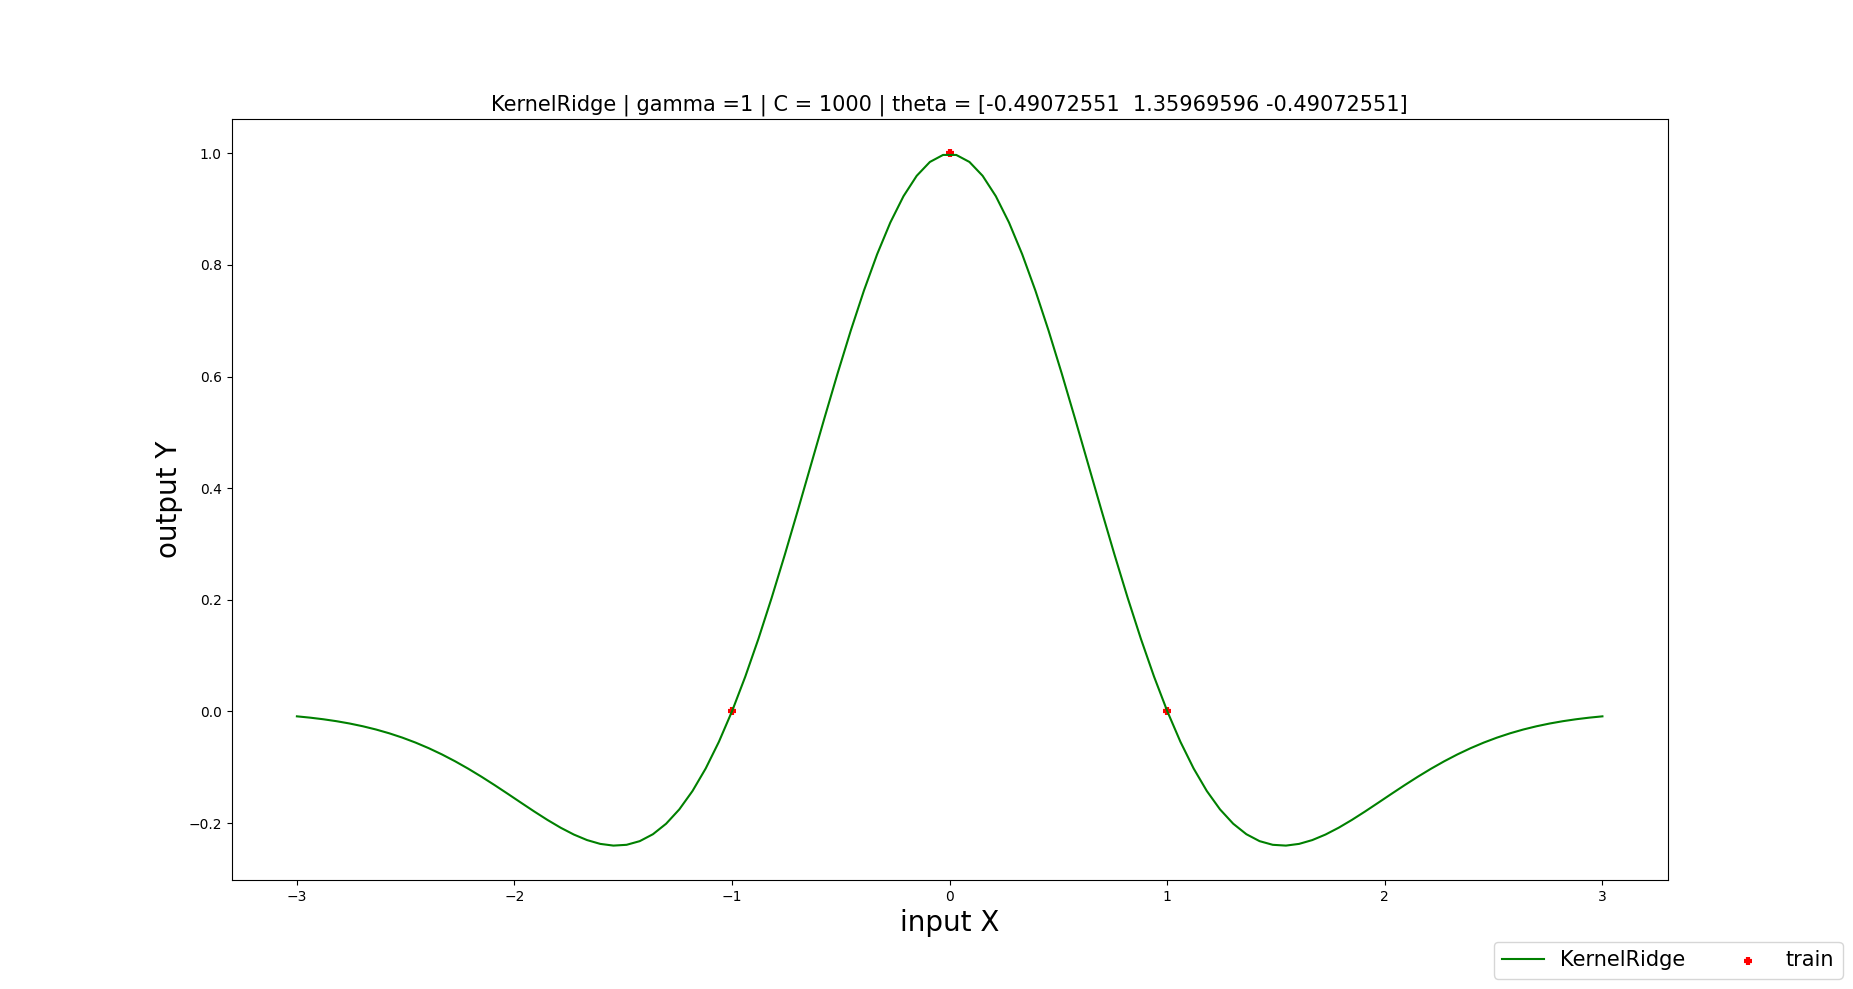
\includegraphics[scale=0.15]{kridge_gamma_1_c_1000.png}}
\end{figure}

$\gamma$ = 5
\begin{figure}[H]    
    \fbox{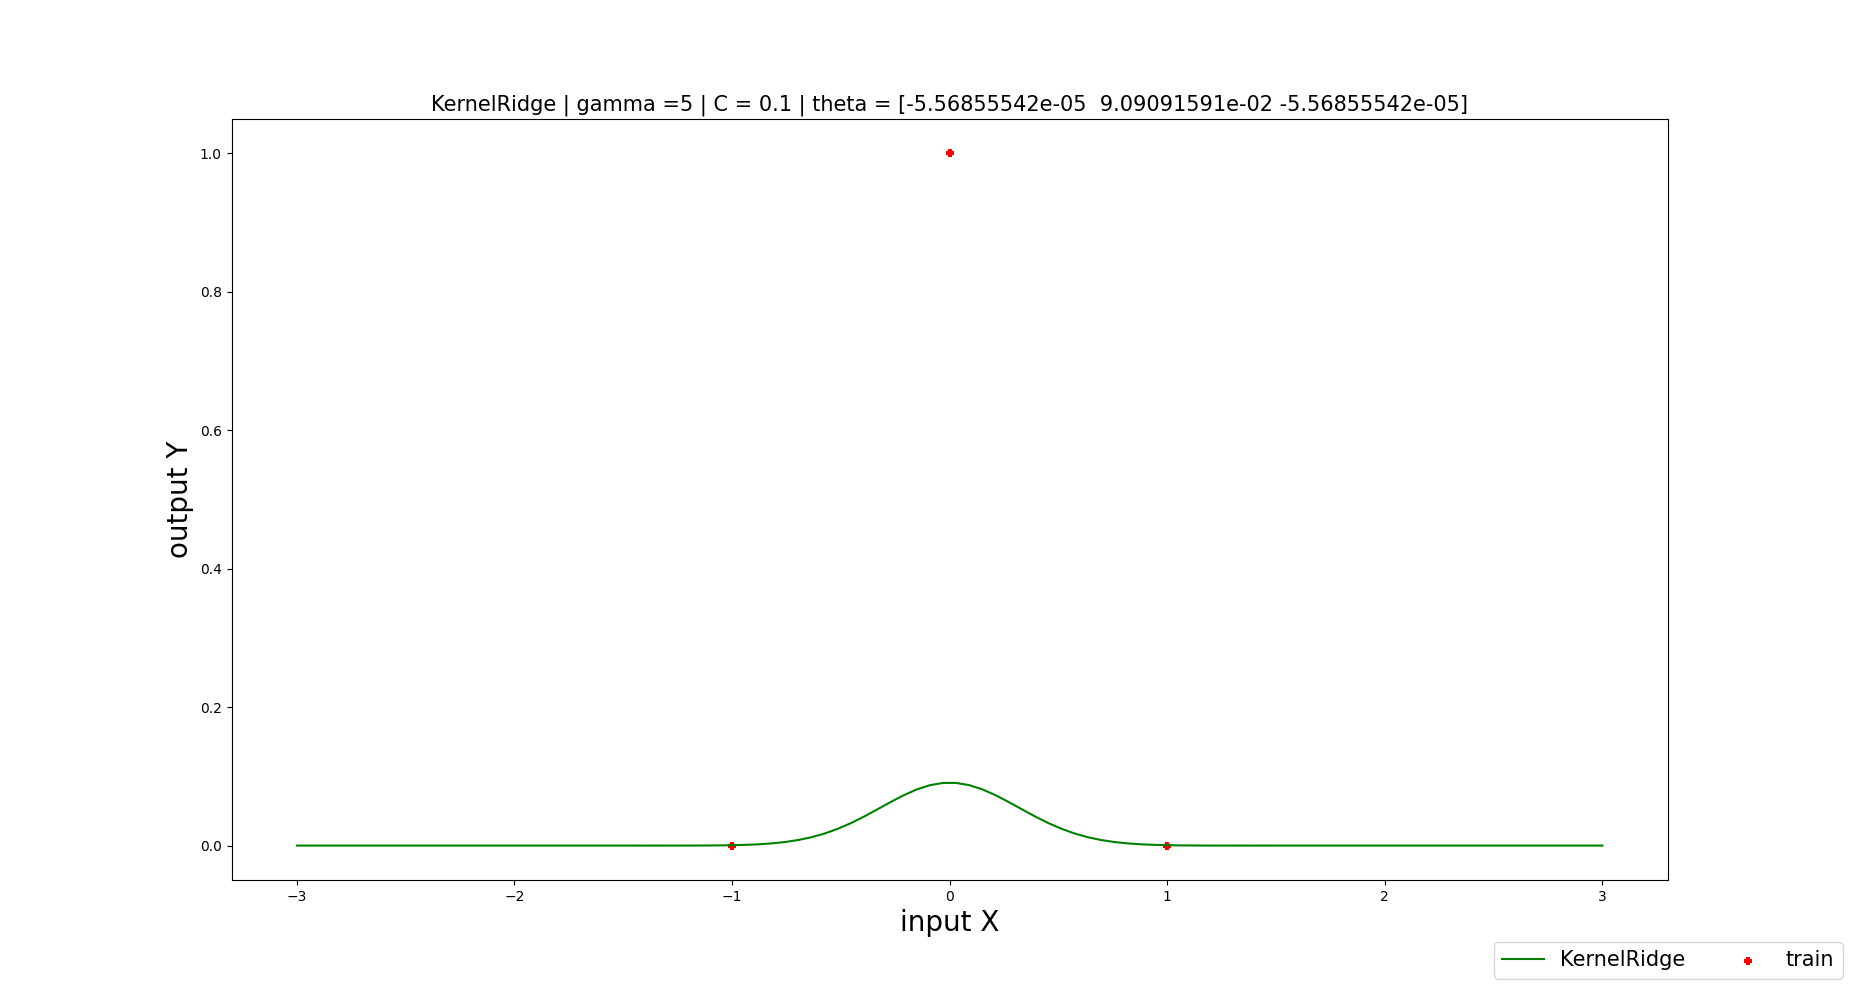
\includegraphics[scale=0.15]{kridge_gamma_5_c_01.png}}   
    \fbox{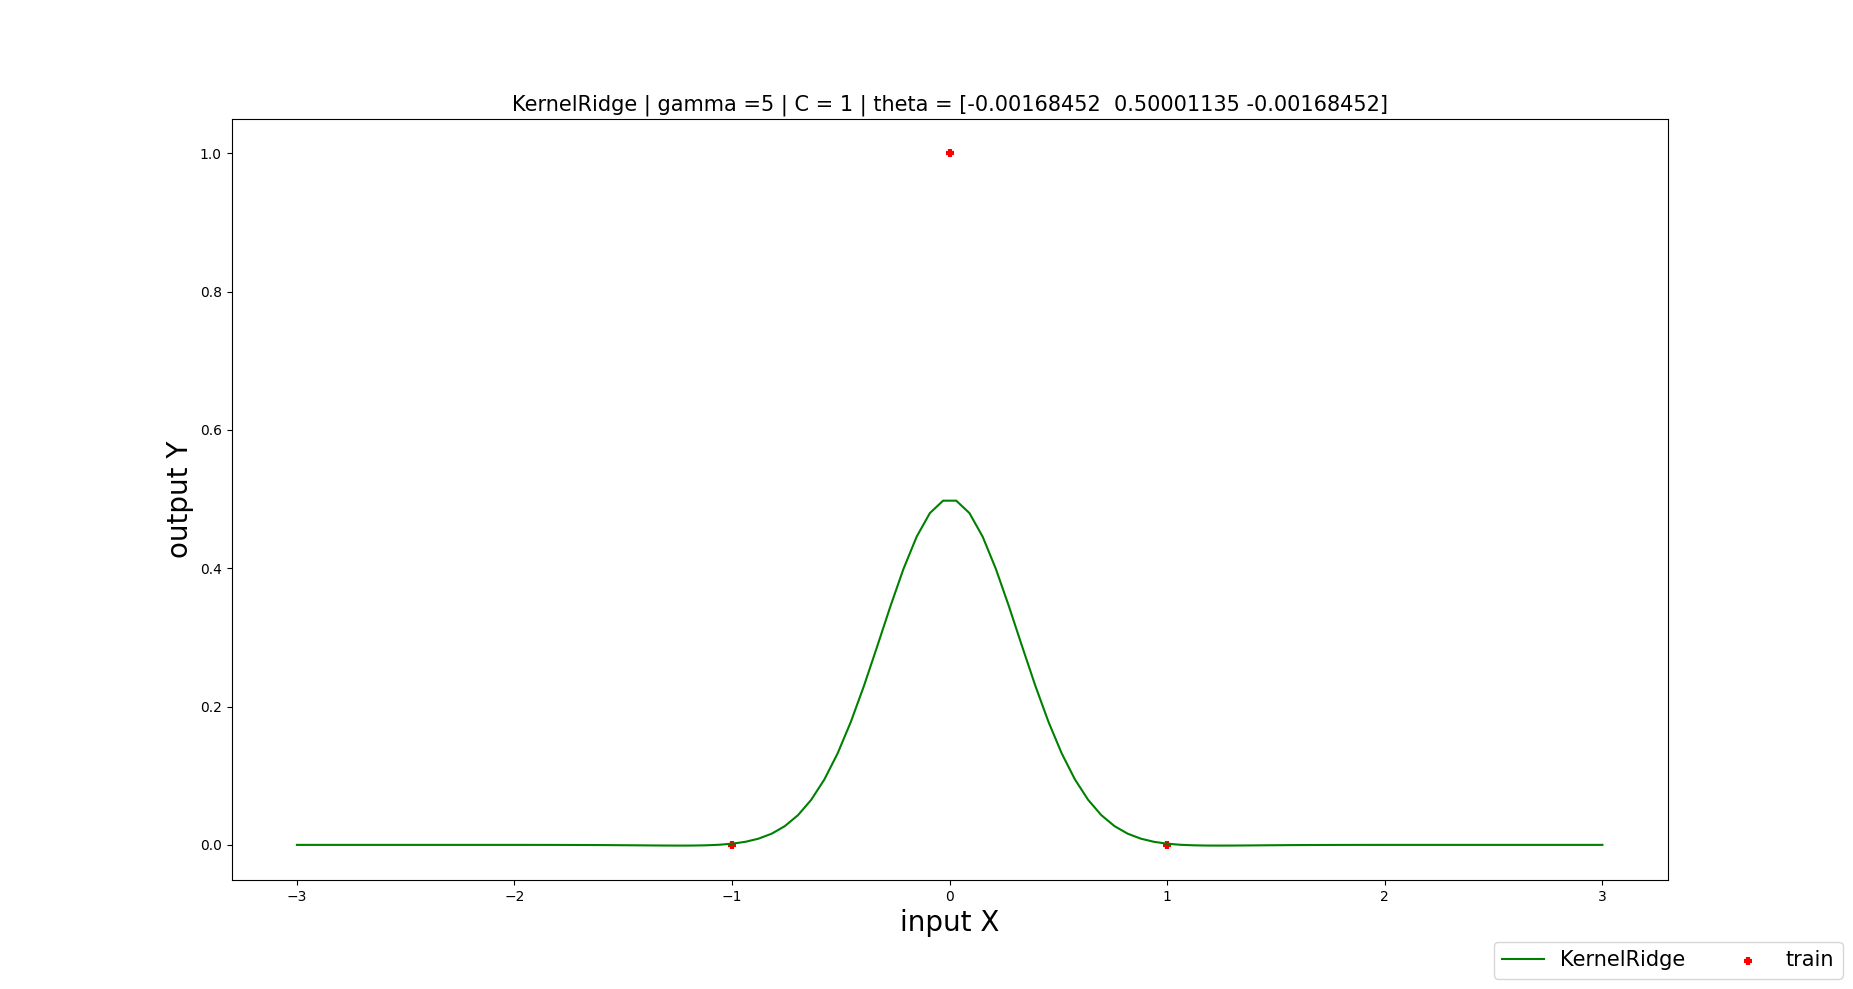
\includegraphics[scale=0.15]{kridge_gamma_5_c_1.png}}   
    \fbox{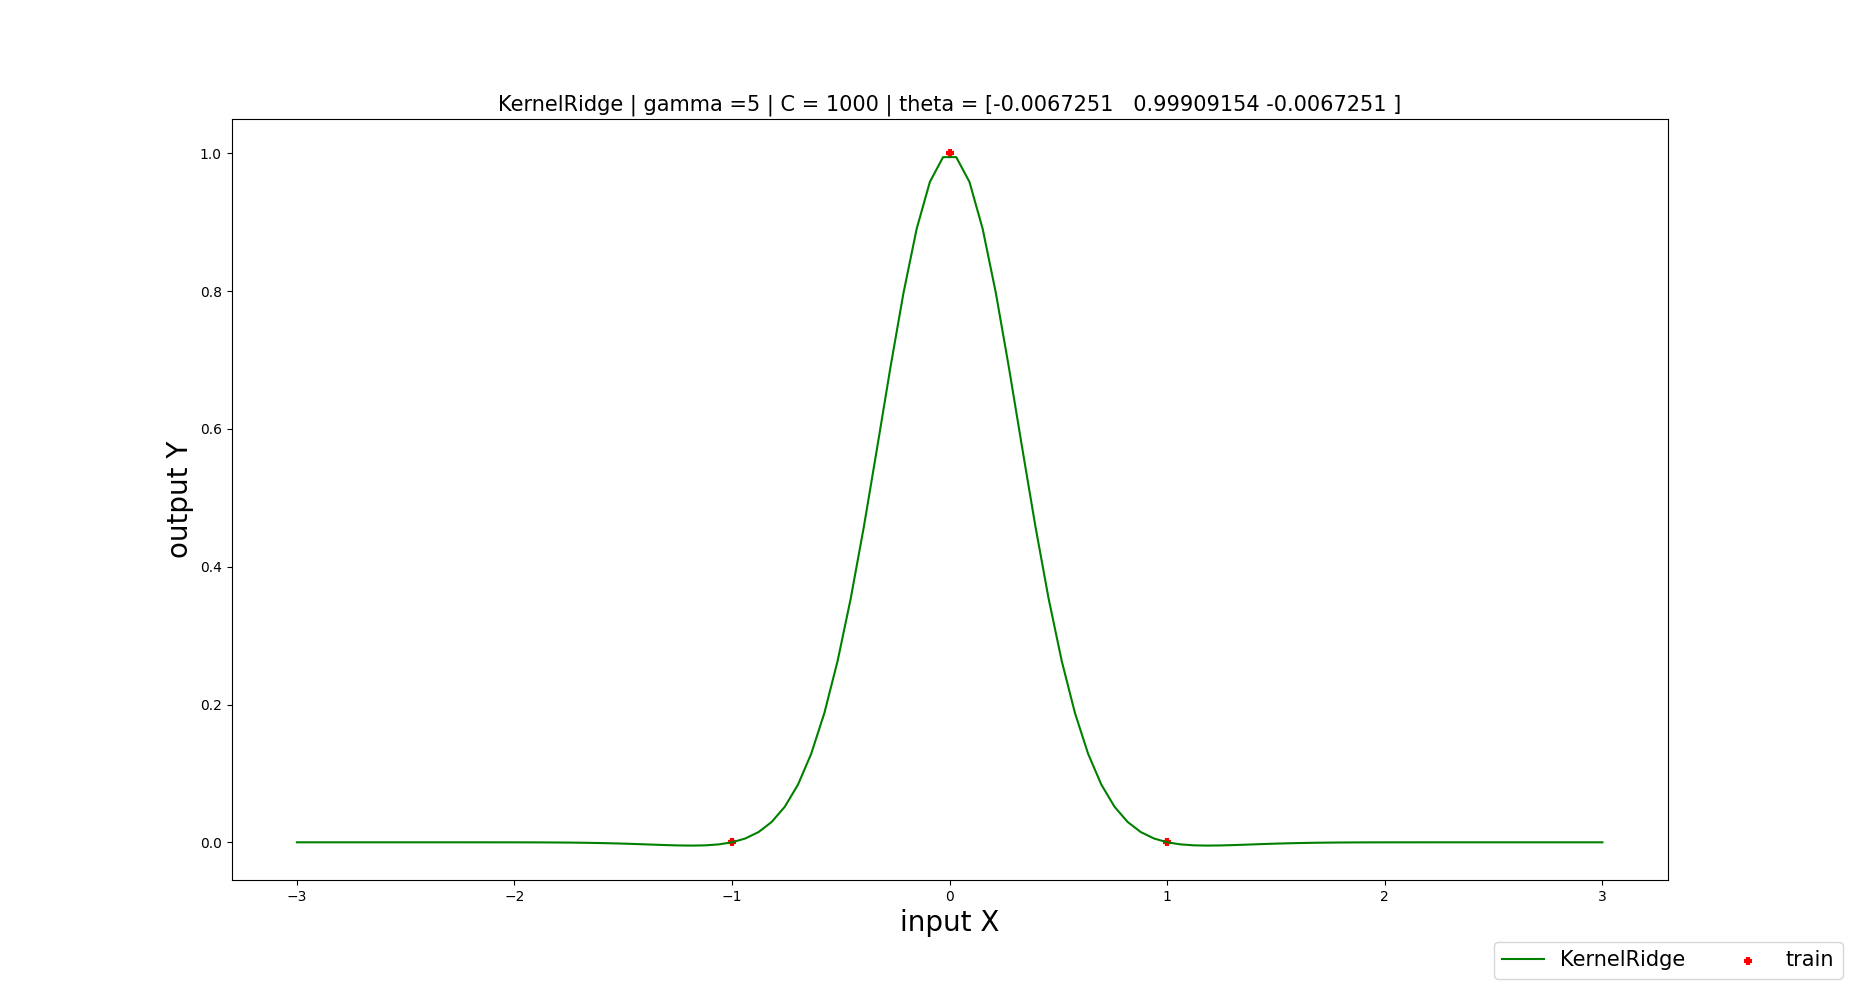
\includegraphics[scale=0.15]{kridge_gamma_5_c_1000.png}}
\end{figure}

$\gamma$ = 10
\begin{figure}[H]    
    \fbox{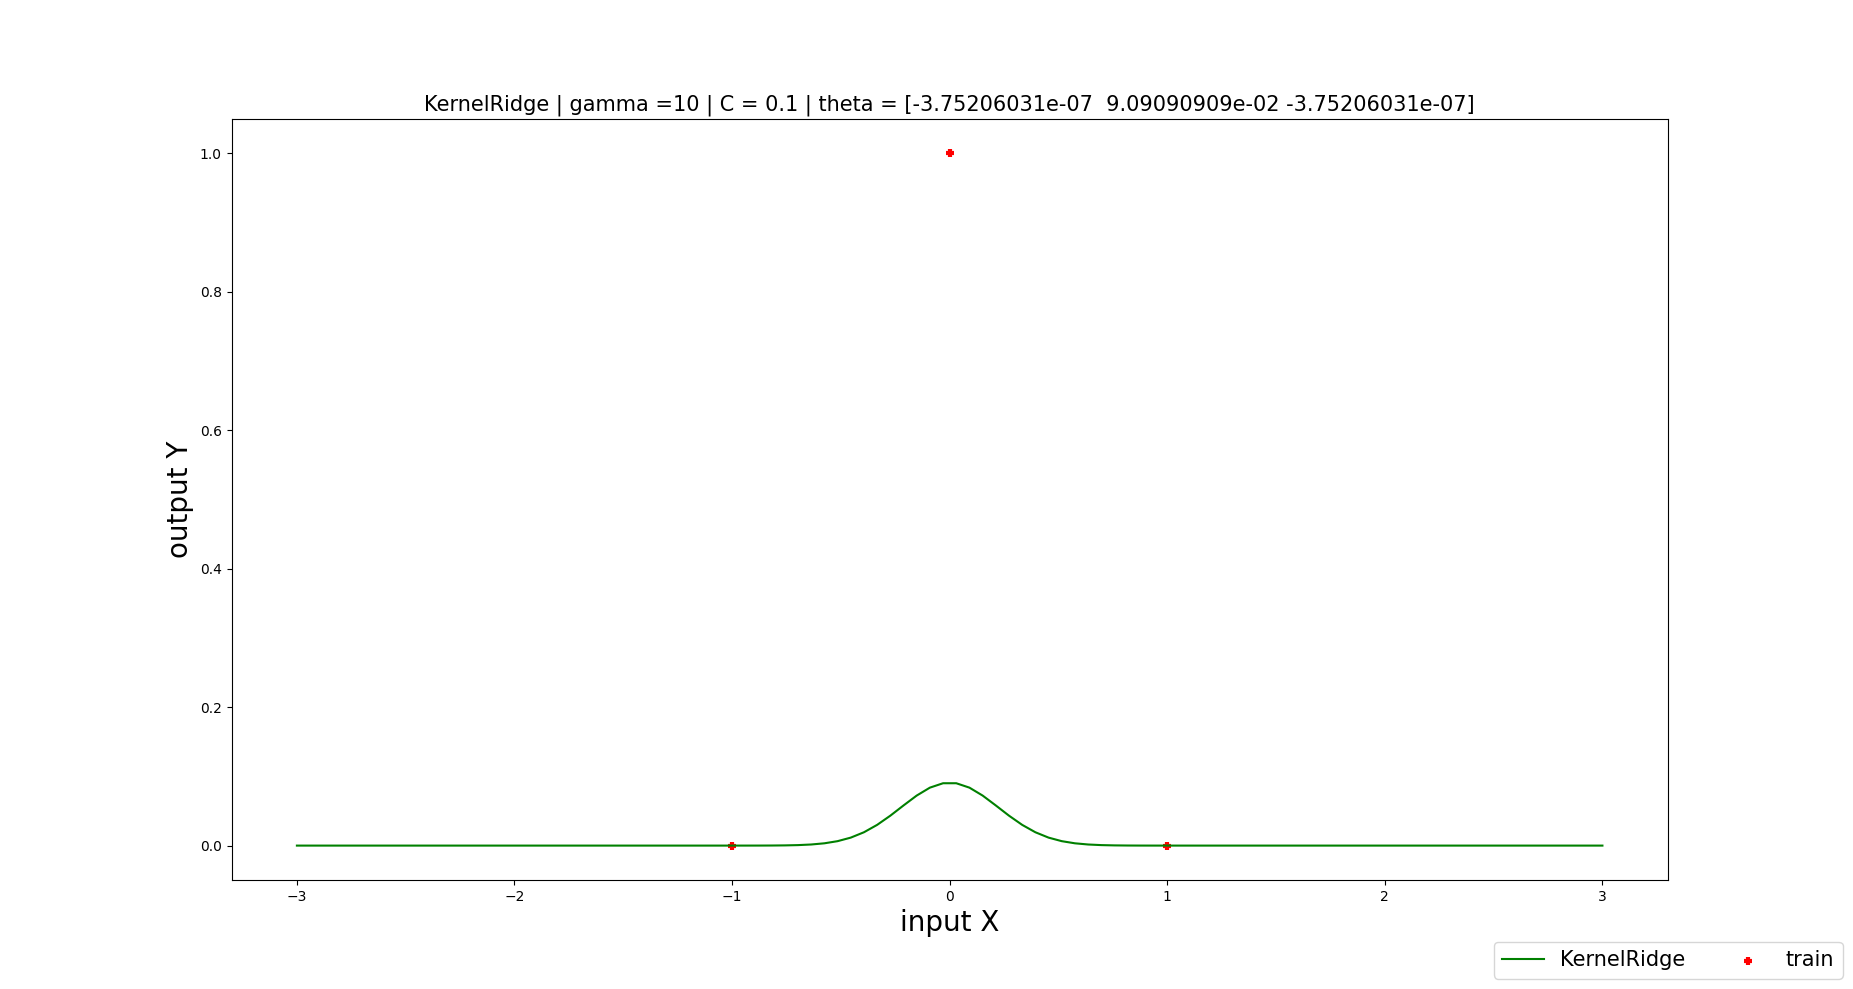
\includegraphics[scale=0.15]{kridge_gamma_10_c_01.png}}   
    \fbox{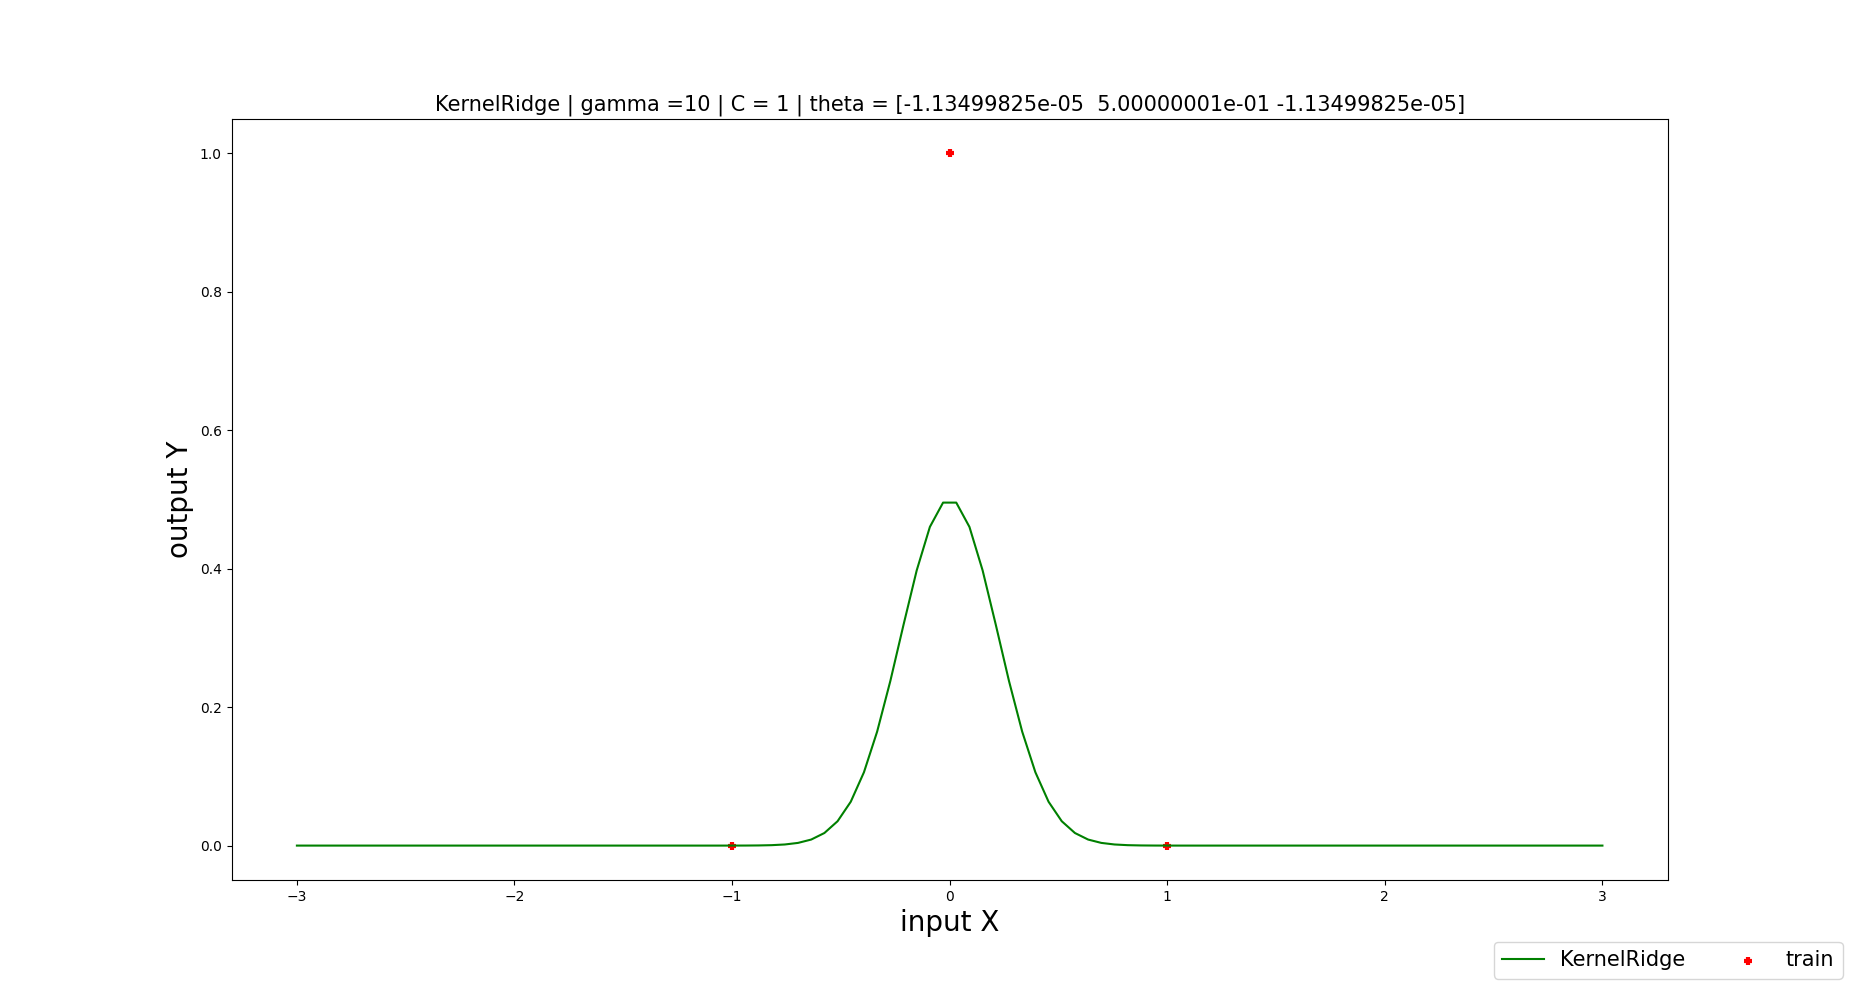
\includegraphics[scale=0.15]{kridge_gamma_10_c_1.png}}   
    \fbox{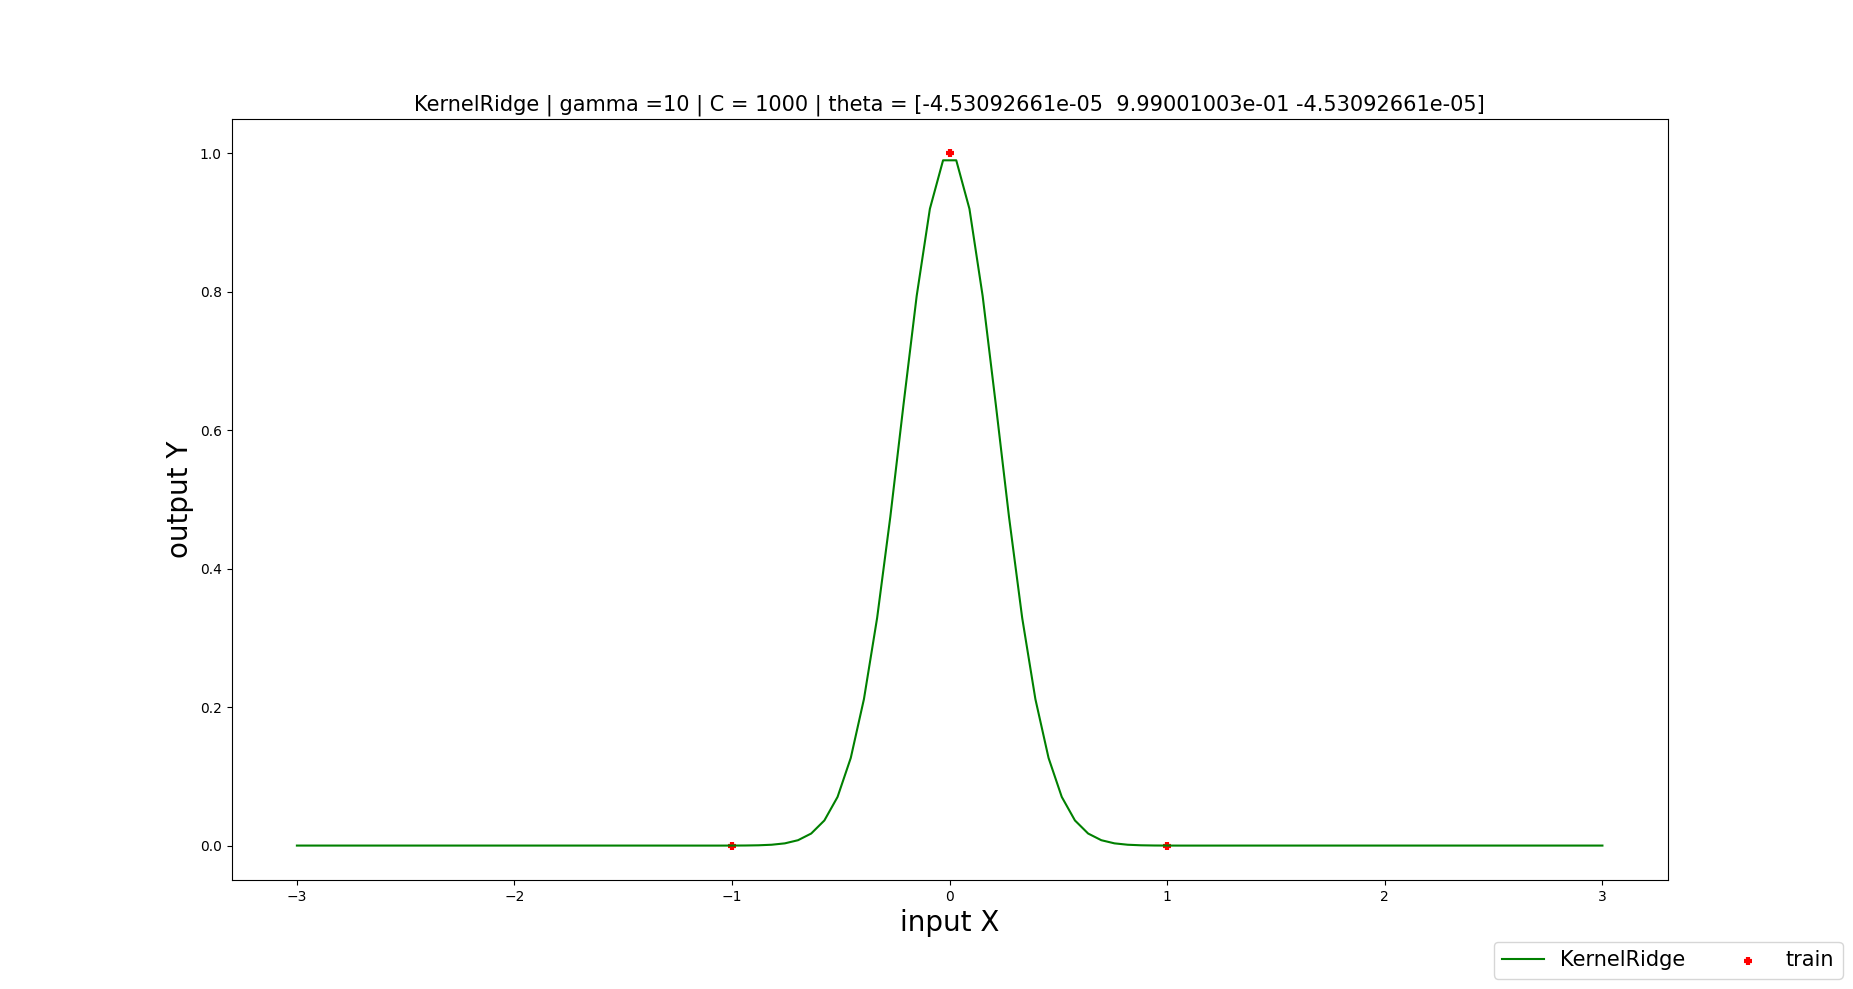
\includegraphics[scale=0.15]{kridge_gamma_10_c_1000.png}}
\end{figure}

$\gamma$ = 25
\begin{figure}[H]    
    \fbox{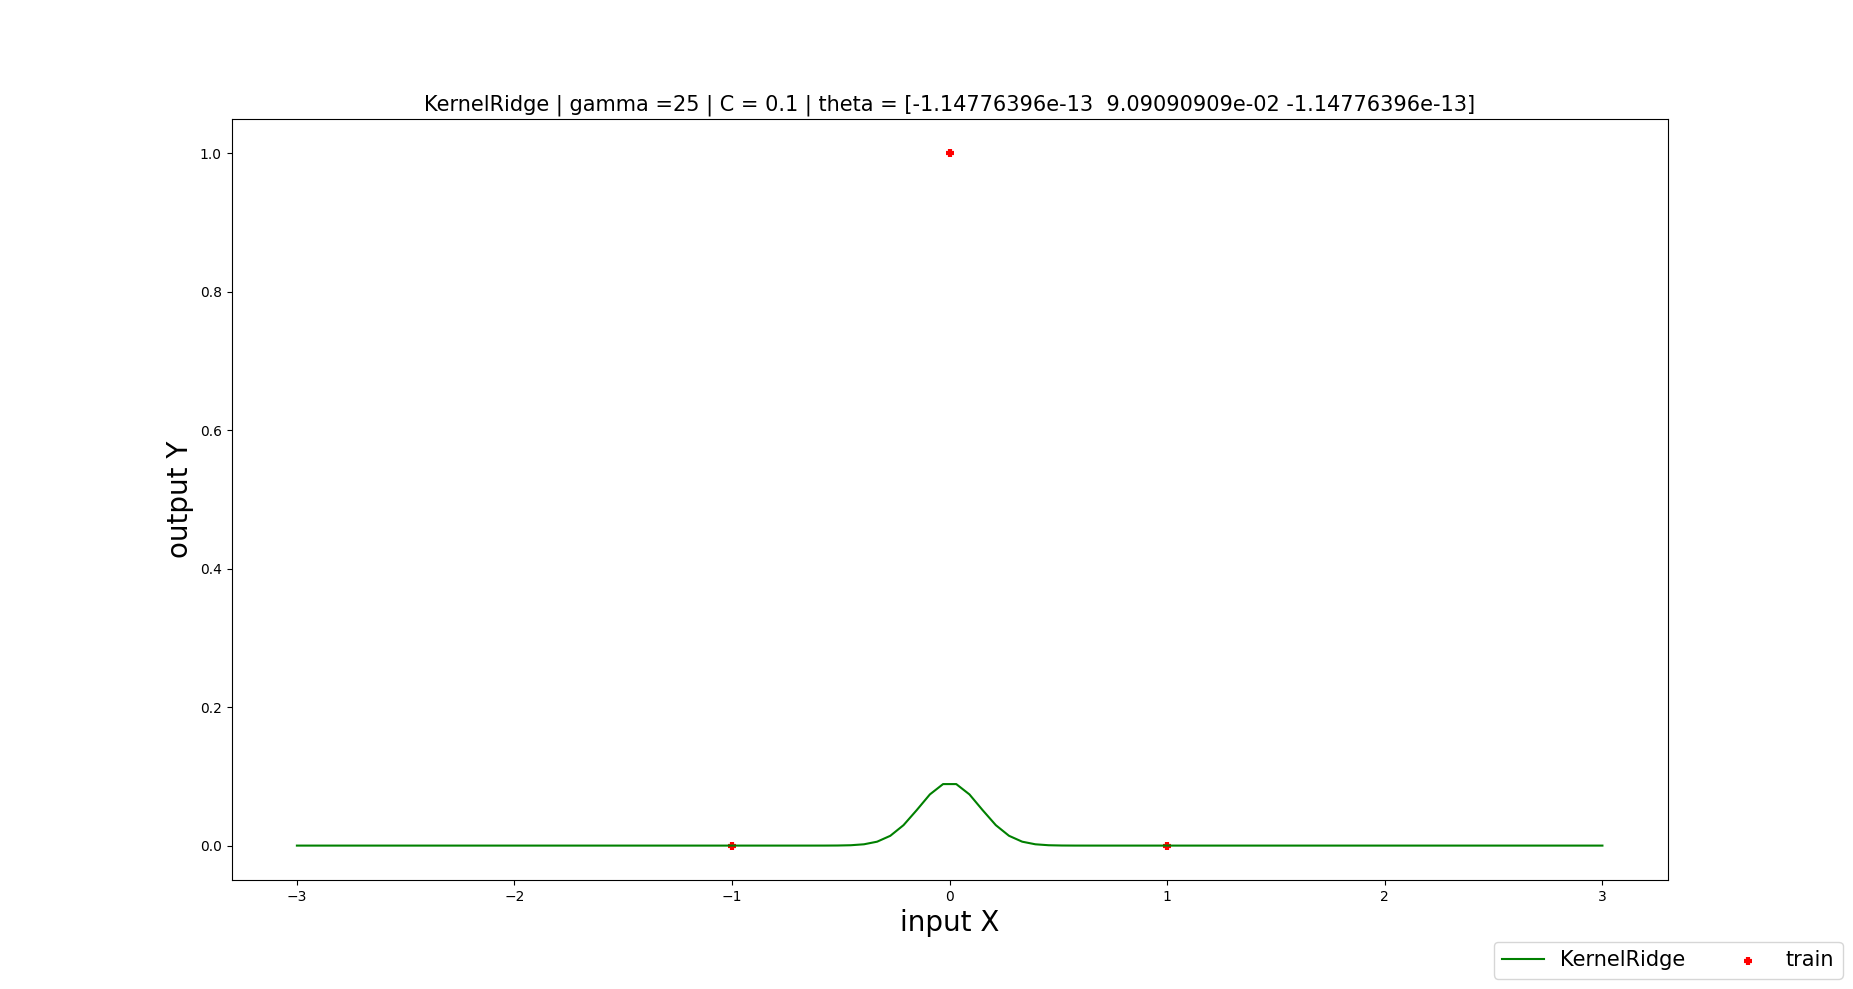
\includegraphics[scale=0.15]{kridge_gamma_25_c_01.png}}   
    \fbox{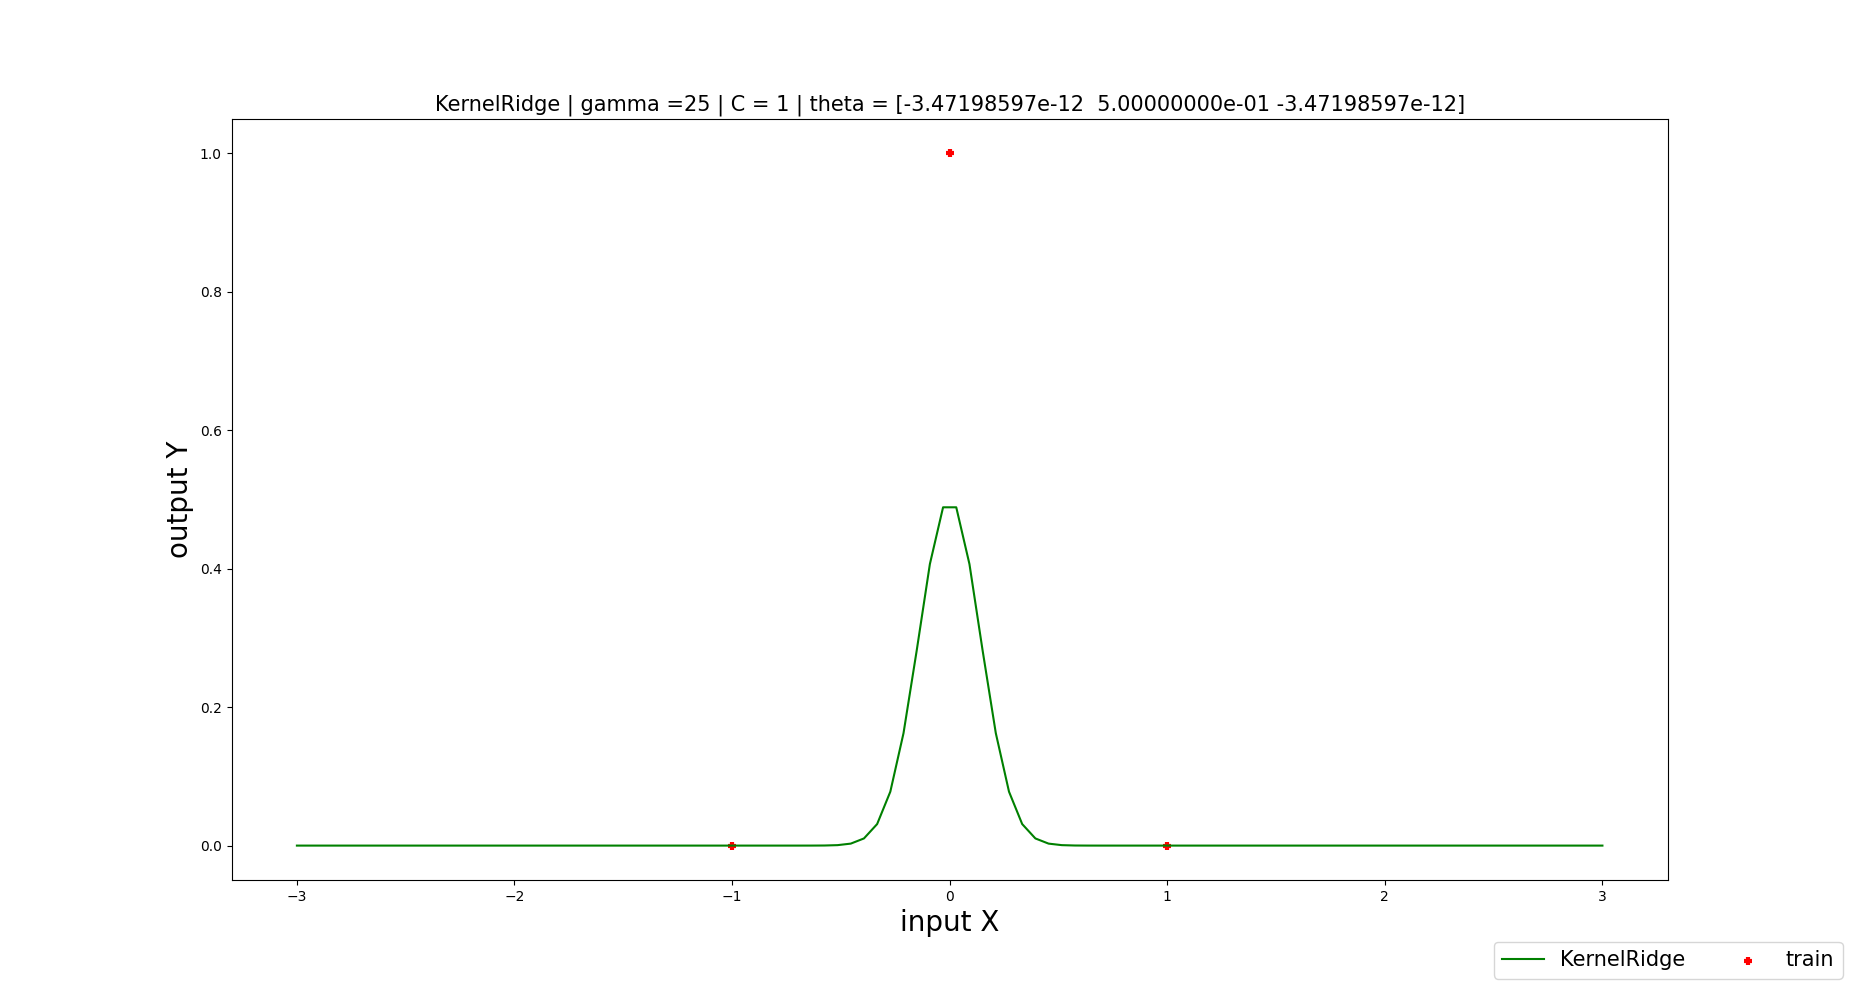
\includegraphics[scale=0.15]{kridge_gamma_25_c_1.png}}   
    \fbox{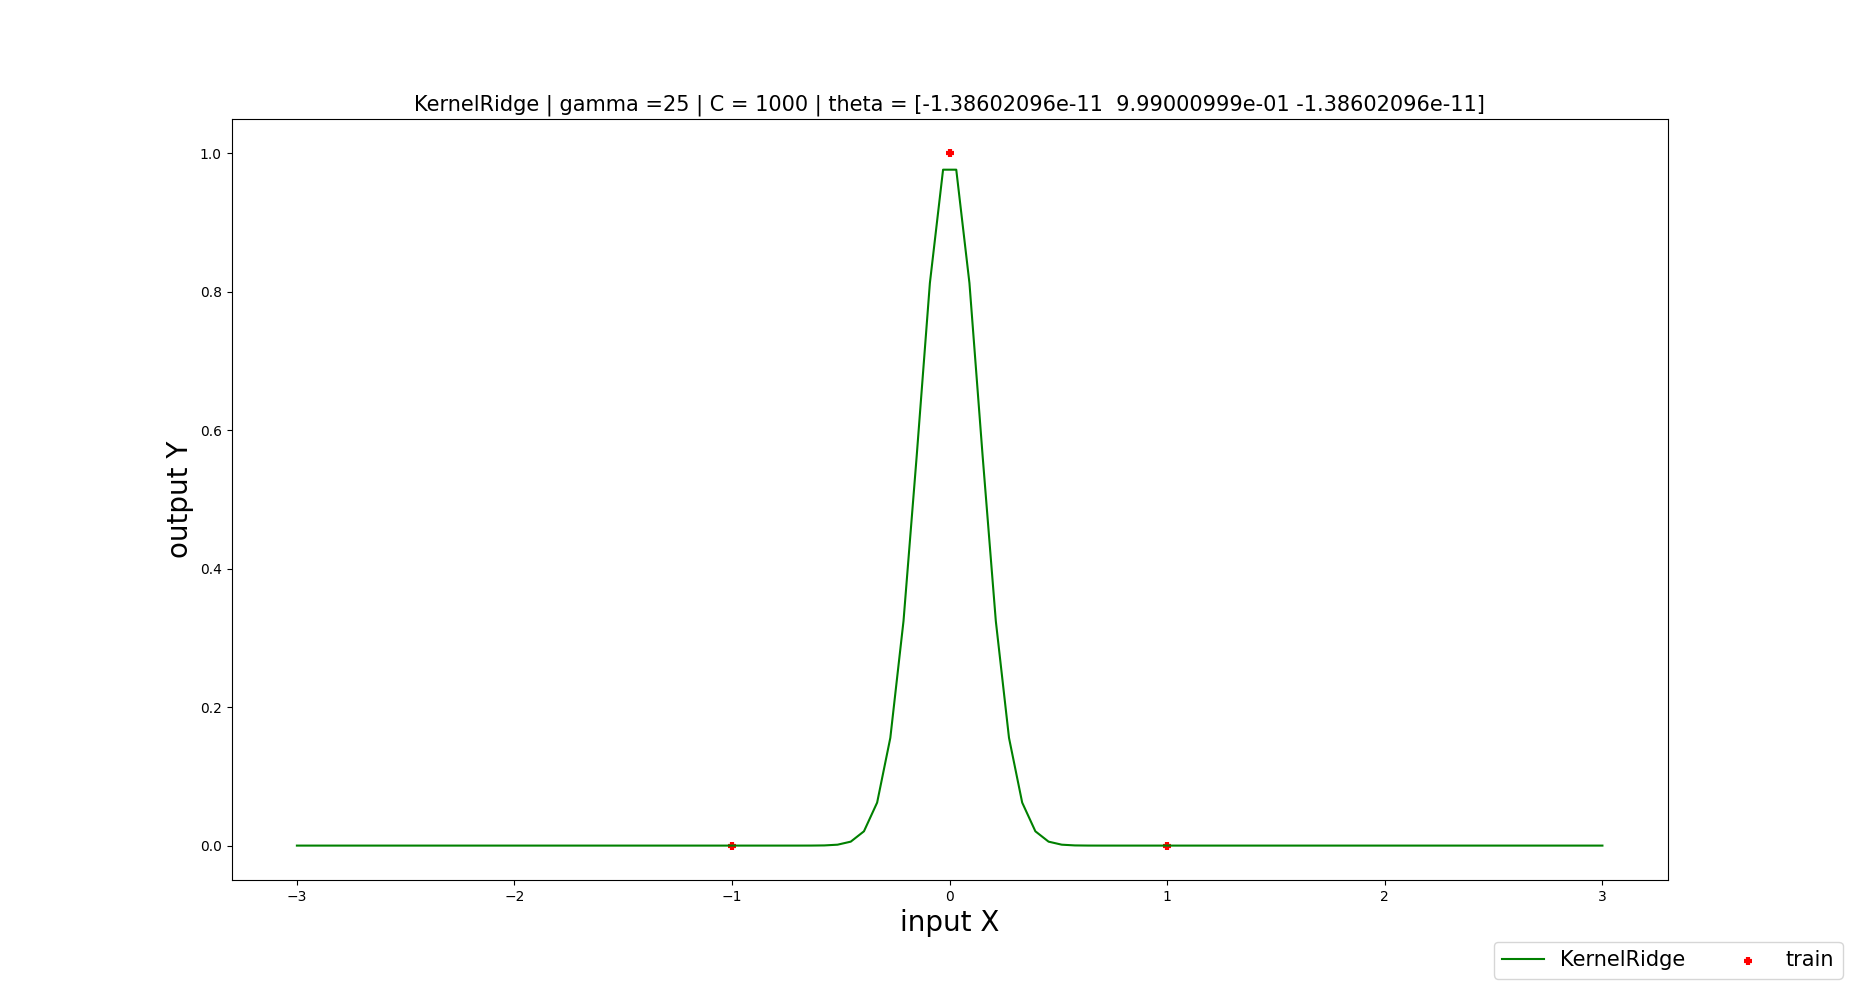
\includegraphics[scale=0.15]{kridge_gamma_25_c_1000.png}}
\end{figure}

\subsection*{Part d}
A kernel ridge regression uses a ridge regression model (that is a model where the loss function is least squares). As mentioned
in the previous question it also uses an L2 penalty, that is its regularisation term is of $\alpha = \frac{1}{2C}$. 
Now, the particularity of a Kernel ridge regression is that it using the "kernel trick", that is using a linear
model to solve a non-linear problem, it essentially maps our features into new, linearly seperable data points. In this
situation we are using a gaussian kernel, that is the KernelRidge's kernel parameter in sklearn is set to 'rbf'.

Let's now look into how predictions change with respect to $\gamma$ and C changing. Starting with varying values for
$\gamma$, we notice that the same observation as we've pointed out for the kNN model applies: as $\gamma$ grows, our 
value for $K(x^{i}, x)$ decreases much faster as the distance between $x^{i}$ and $x$ grows, thus, once again we can see
that small values of $\gamma$ see small fluctuations over a large part of the range of x values, while large values such 
as $\gamma = 25$ go from a low predictiong to a high predictions very fast, over a very small distance (or range) of x.

\vspace{5mm} %5mm vertical space

In terms of varying our C value, we can take any value of $\gamma$ as a reference given we notice the same trend,
a very low value for C such as 0.1 will enable for very small fluctuations of predictions, and that fluctuation will
increase as C does too. This makes sense as instead of optimising for simply the loss function, we try to minimize the
loss + the penalty term. Thus when C is very small, $\alpha$ is very large, thus making the penalty term very big we
obtain very little variation. When C is very large, $\alpha$ is very small thus that penalty term is not as impactful
and our model will have more variations based on the data it is trained with.

\vspace{5mm} %5mm vertical space

Looking at $\theta$ from the title of these graphs, we notice a few trends. Throughout, we see that as C becomes bigger,
so do the coefficients, taking $\gamma = 5$ as an example we have: $\theta = $ $-5.5 * 10^{-5}$, $9*10^{-2}$ and $-5.56*10^{-5}$ 
when $C = 0.1$, and when $ C = 1000$ : $\theta = - 0.0067$, $1$ and $-0.0067$ (roughly). And the same is noticeable for the other
values of $\gamma$.

Finally, we also notice that as $\gamma$ gets biggers, our coefficients become smaller, having for example:
$\theta = -333, 666, -333$ when $\gamma = 0$ and $C = 1000$, and when $\gamma = 25$ and $C = 1000$ : 
$\theta = 1.38 * 10^{-11}, 0.99, -1.38 * 10^{11}$.


\section{Question ii}
\subsection*{Part a}
Let's first clarify the range I have used for testing my models; I decided to follow the trend as suggested 
by the exercise and the went with the range $[- 3 * abs(min), 3 * max]$. In practise though,
the minimum was a negative value thus I only have to use $[3 * min, 3 * max]$.  

The method is the same as explained in question i thus I will not go over the explaining here. Using the provided
dataset, $ k = \# points in dataset$ and a range for $\gamma = [0, 1, 5, 10, 25]$, we obtain the following predictions after
training a kNN model:

\begin{figure}[H]    
    \fbox{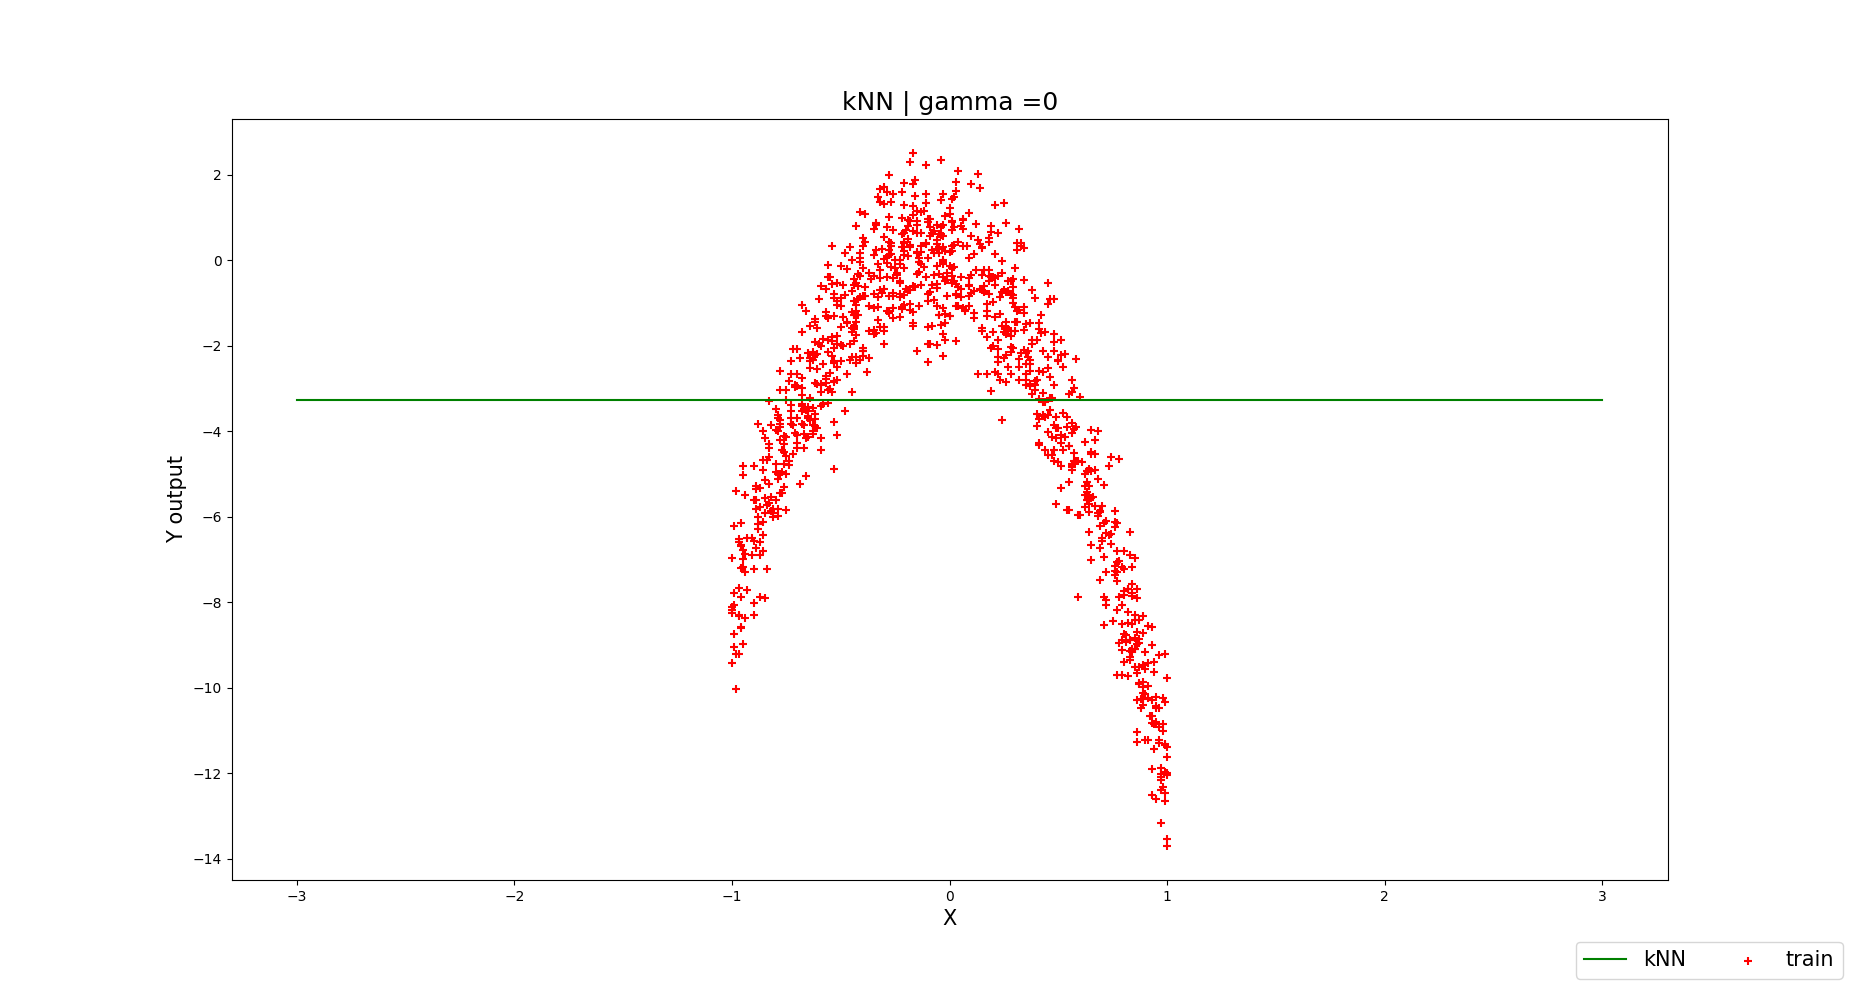
\includegraphics[scale=0.15]{2_knn_gamma_0.png}}   
    \fbox{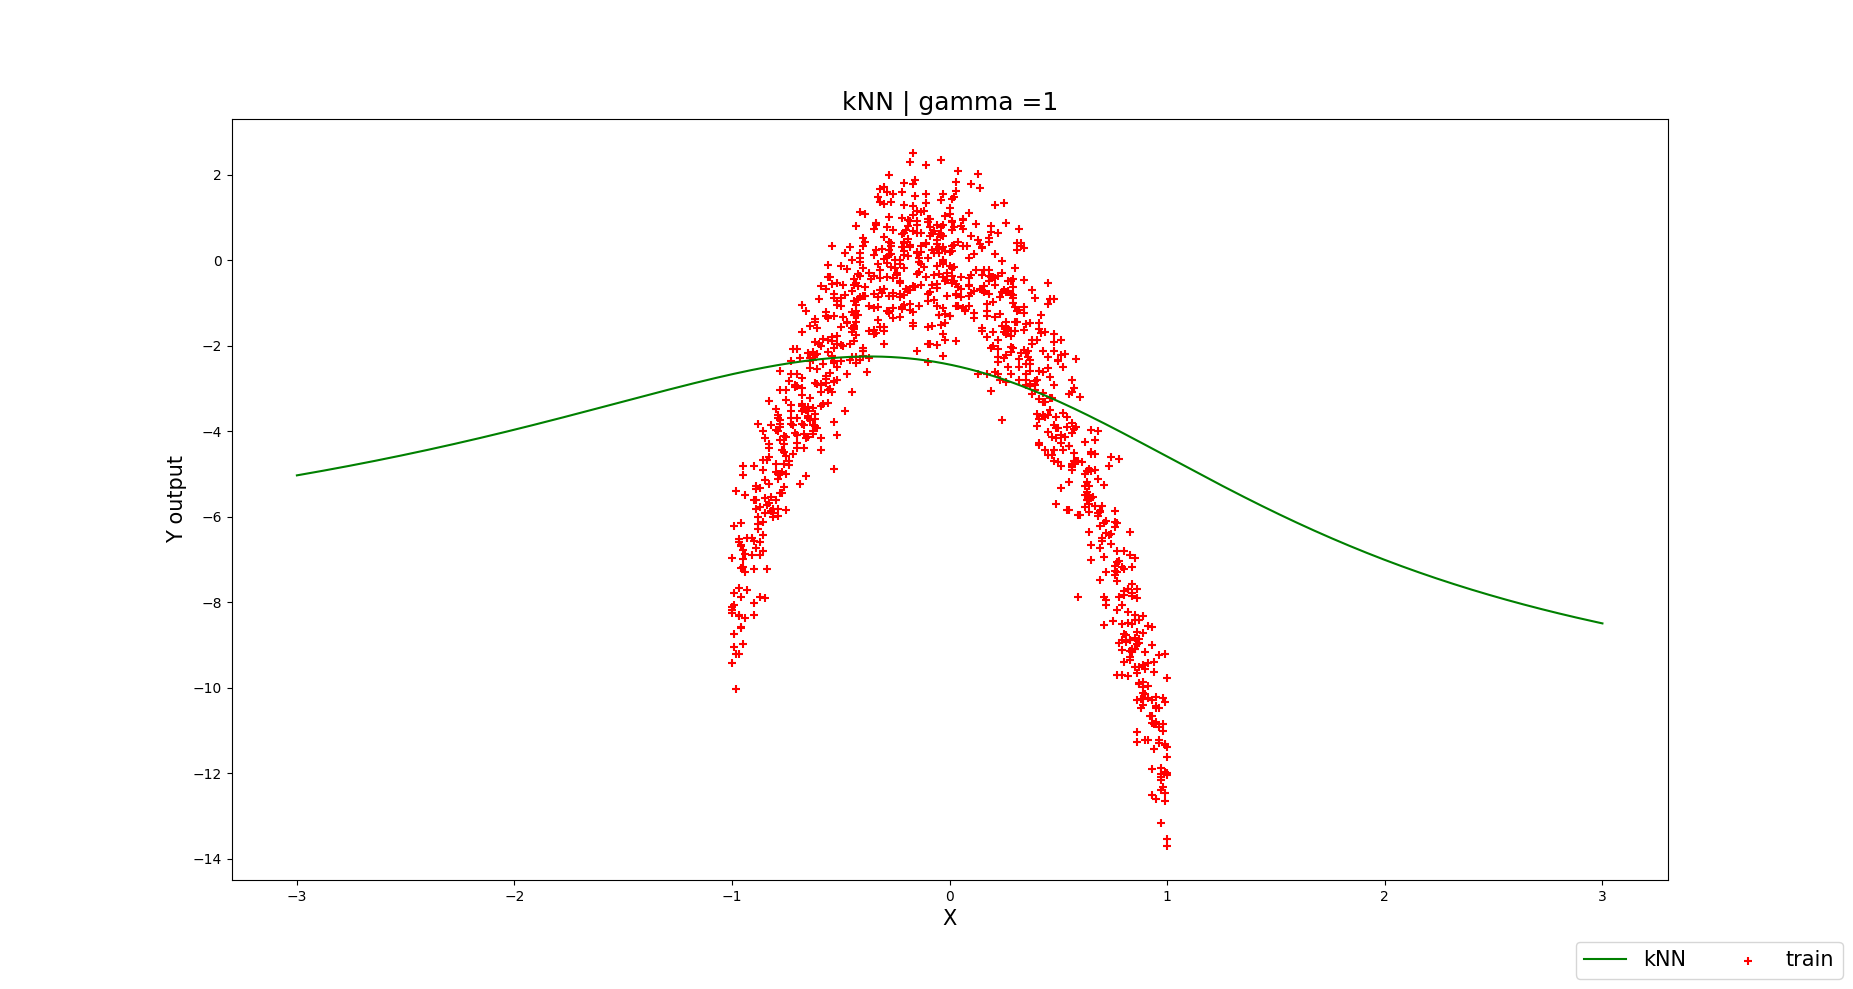
\includegraphics[scale=0.15]{2_knn_gamma_1.png}}   
    \fbox{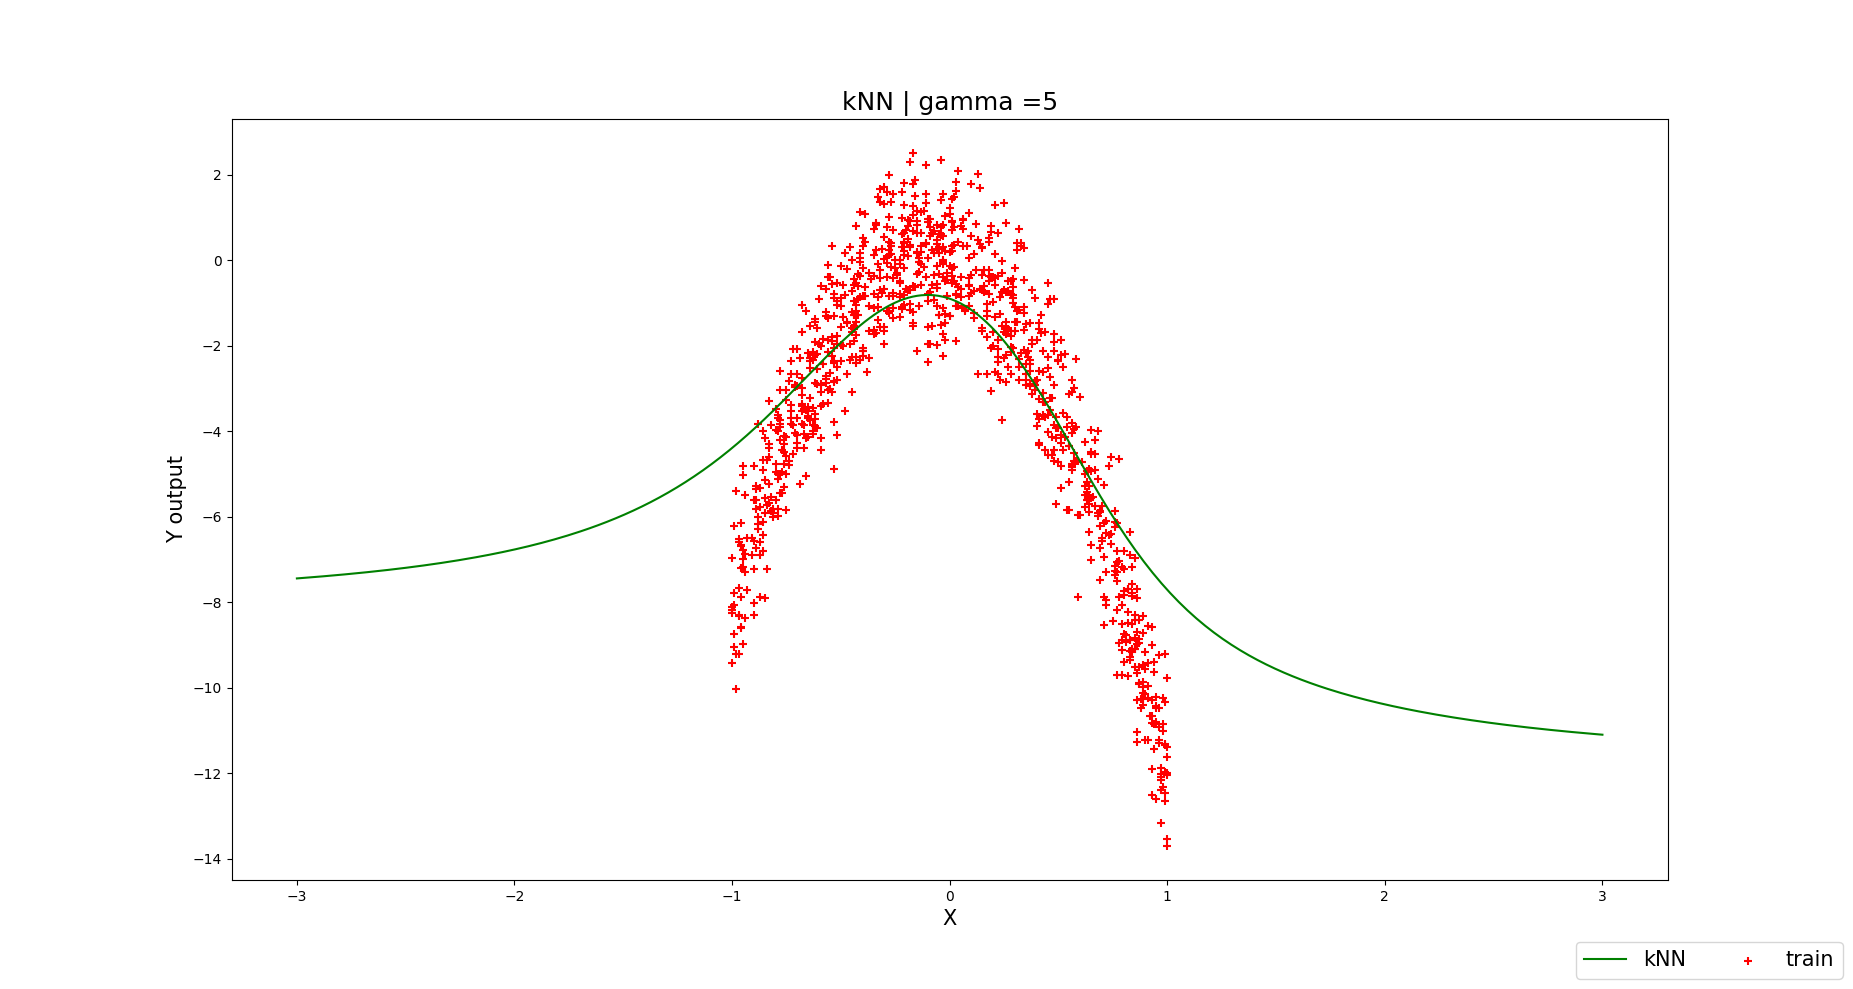
\includegraphics[scale=0.15]{2_knn_gamma_5.png}}
    \fbox{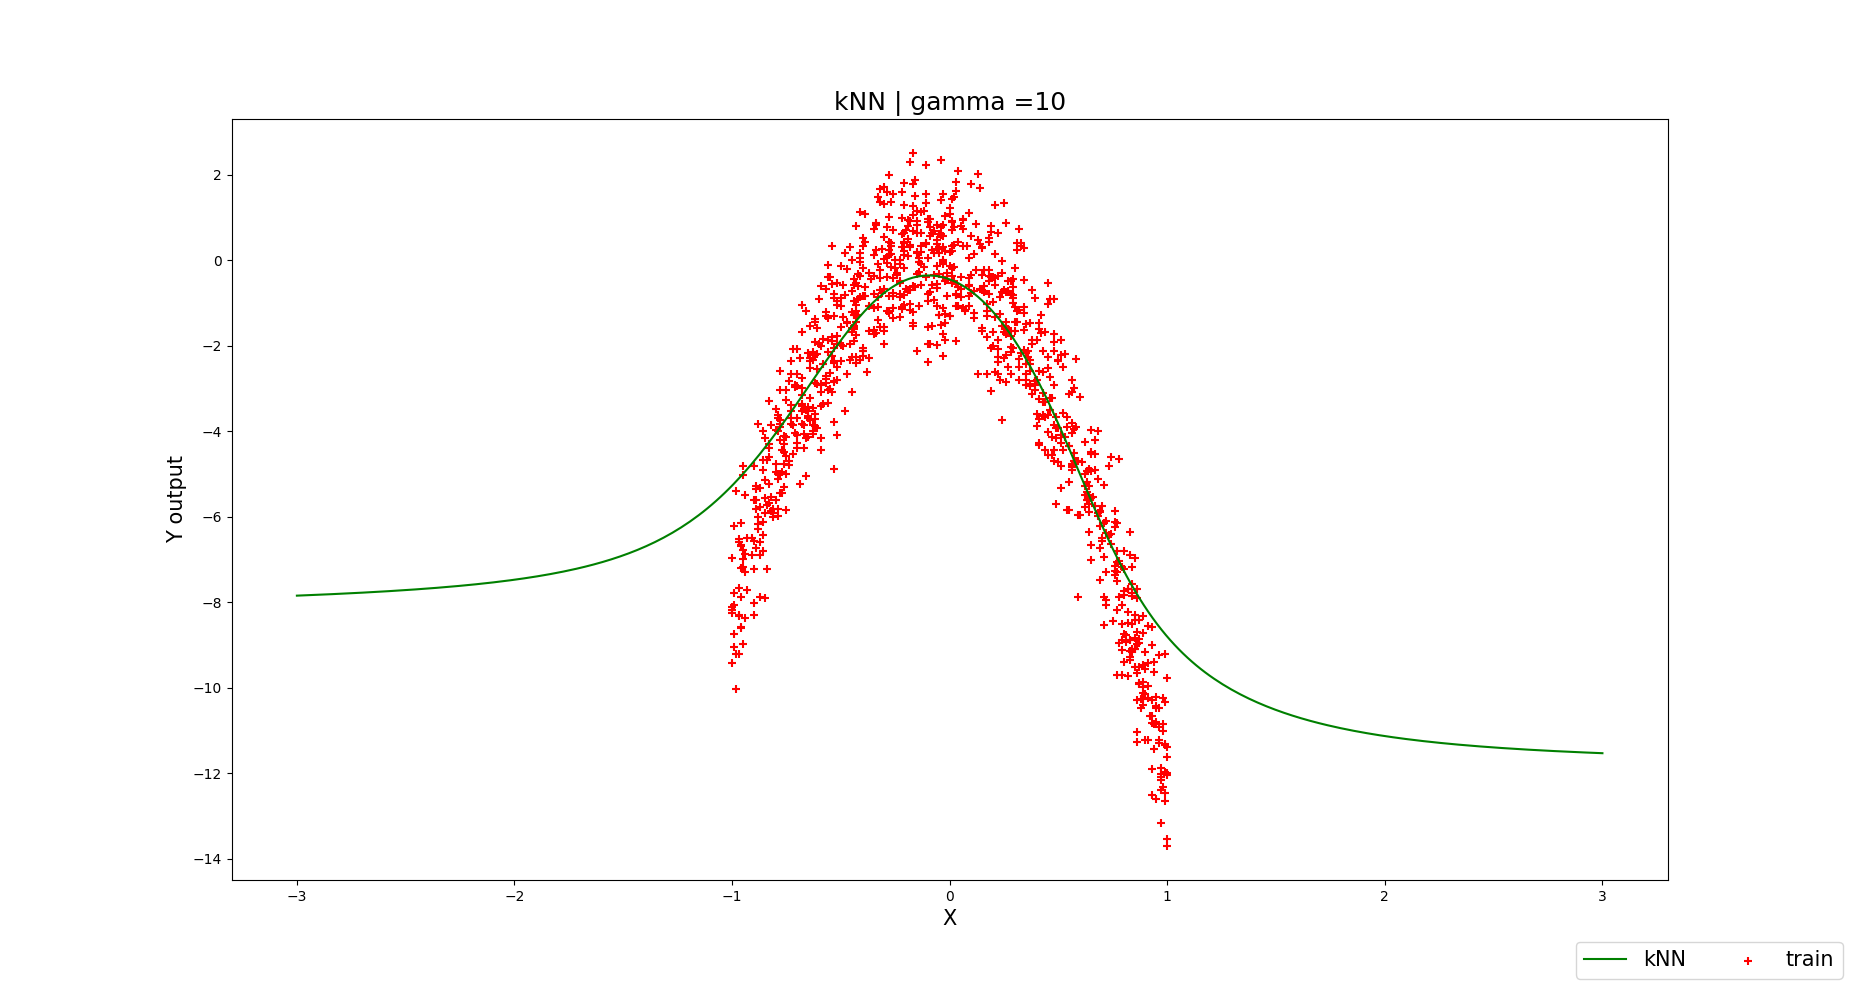
\includegraphics[scale=0.15]{2_knn_gamma_10.png}}
    \fbox{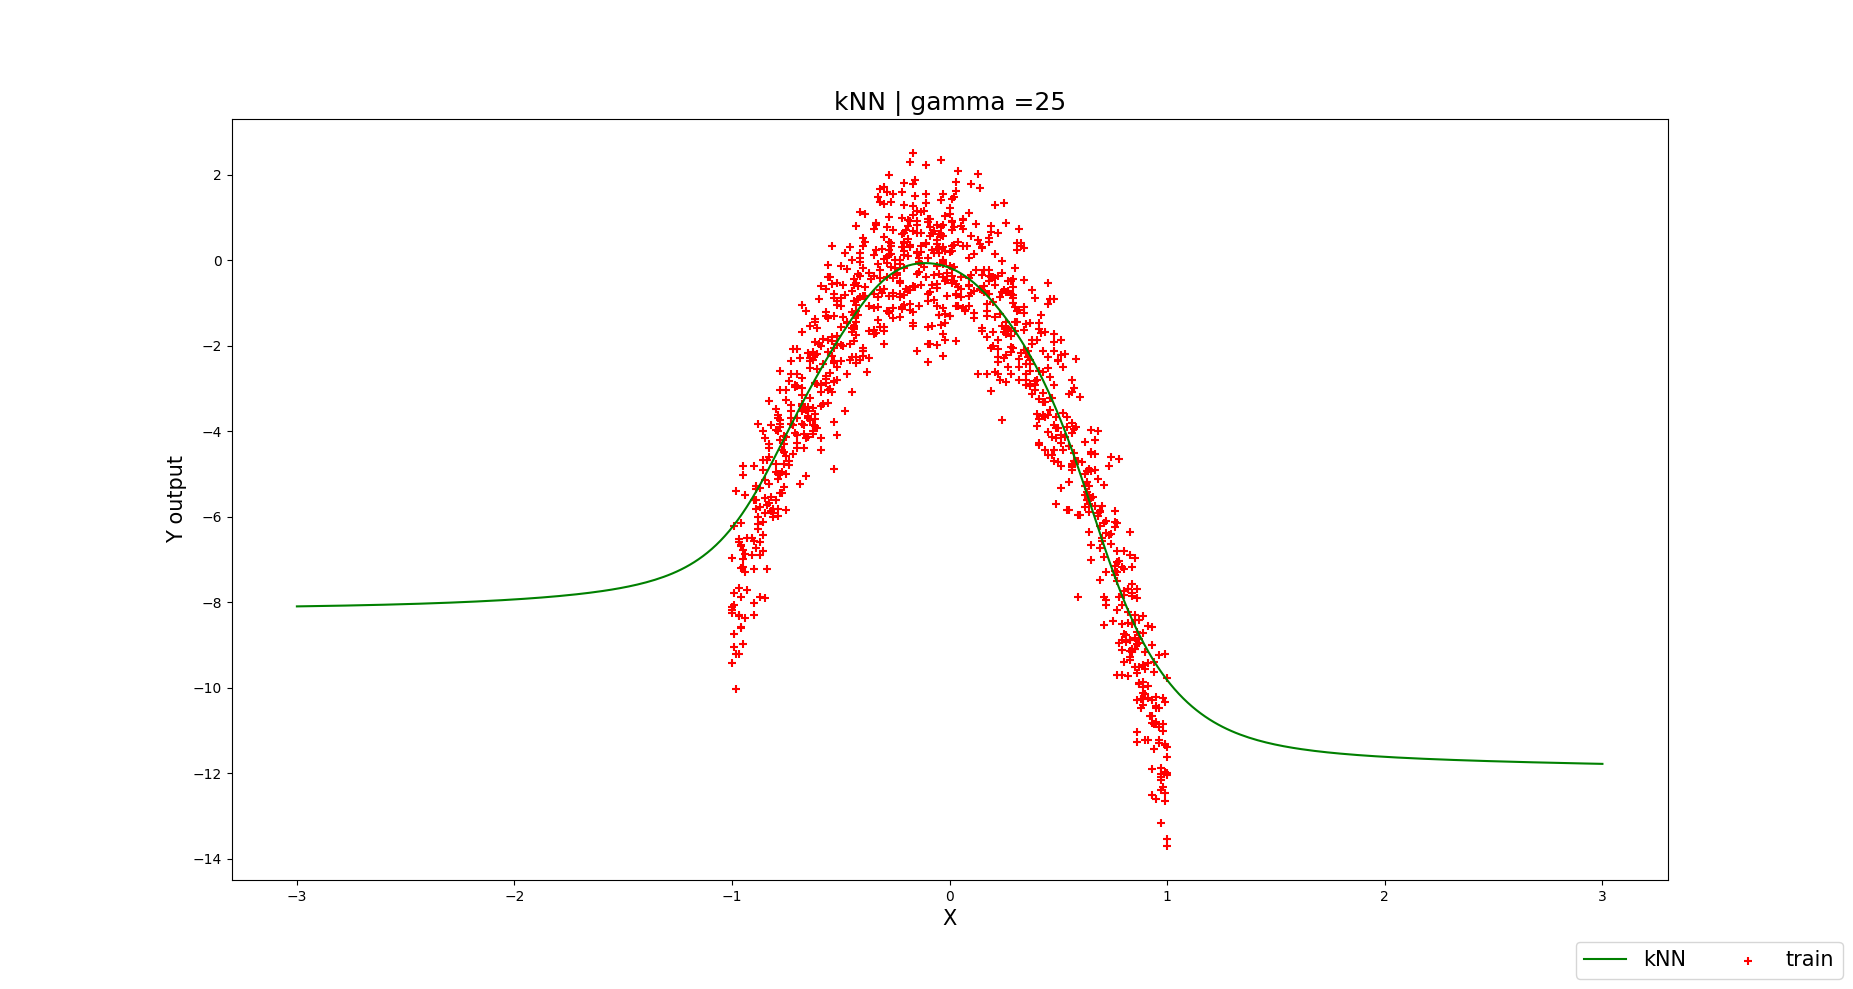
\includegraphics[scale=0.2]{2_knn_gamma_25.png}}
\end{figure}


As mentioned twice before, we notice the same behavior as $\gamma$ grows, the prediction plot
adapts much faster to the data it is trained with, going from starting to follow a trend with $\gamma = 1$
to fitting quite well the training data when $\gamma = 25$.

In terms of how the models generalise outside of the trained data range, we notice that most models
are quite flat looking, with the one for $\gamma = 25$ matching most of the taining data's curve but still flattening out
a bit later, which, given the look of the training data is likely not what would happen.n fact it seems slightly
wrong to try expand the range for this training data as it clearly seems to be set within a set interval of
x values.

\subsection*{Part b}
Similarly to our previous question I have explained most of how this works already so I will not go into details 
again, using the provided dataset as the training data and making the model predict values over the range we
have previously set of $[3 * min, 3 * max]$. We can train KernelRidge models with varying values of $\gamma$.
This question does not mention the loss parameter $C$ at all thus I will use sklearn's default value, which is 1.
We obtain the following plots:

\begin{figure}[H]    
    \fbox{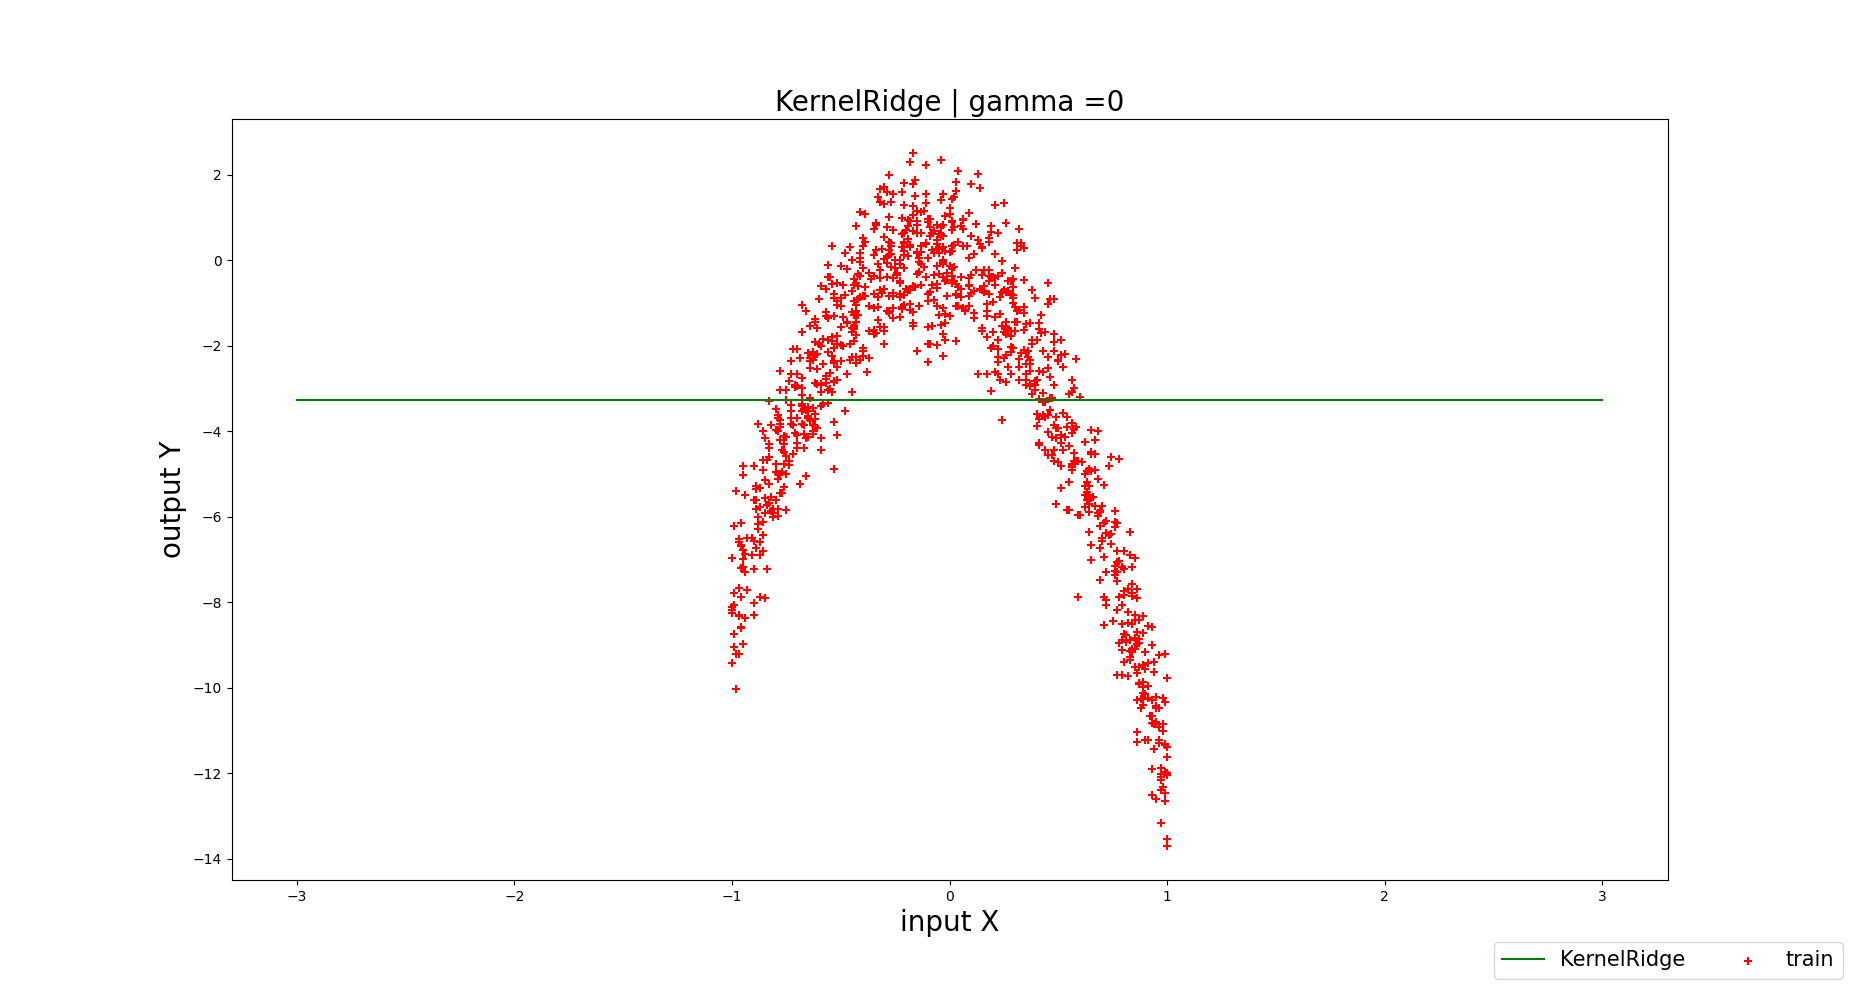
\includegraphics[scale=0.15]{2_kride_gamma_0.png}}   
    \fbox{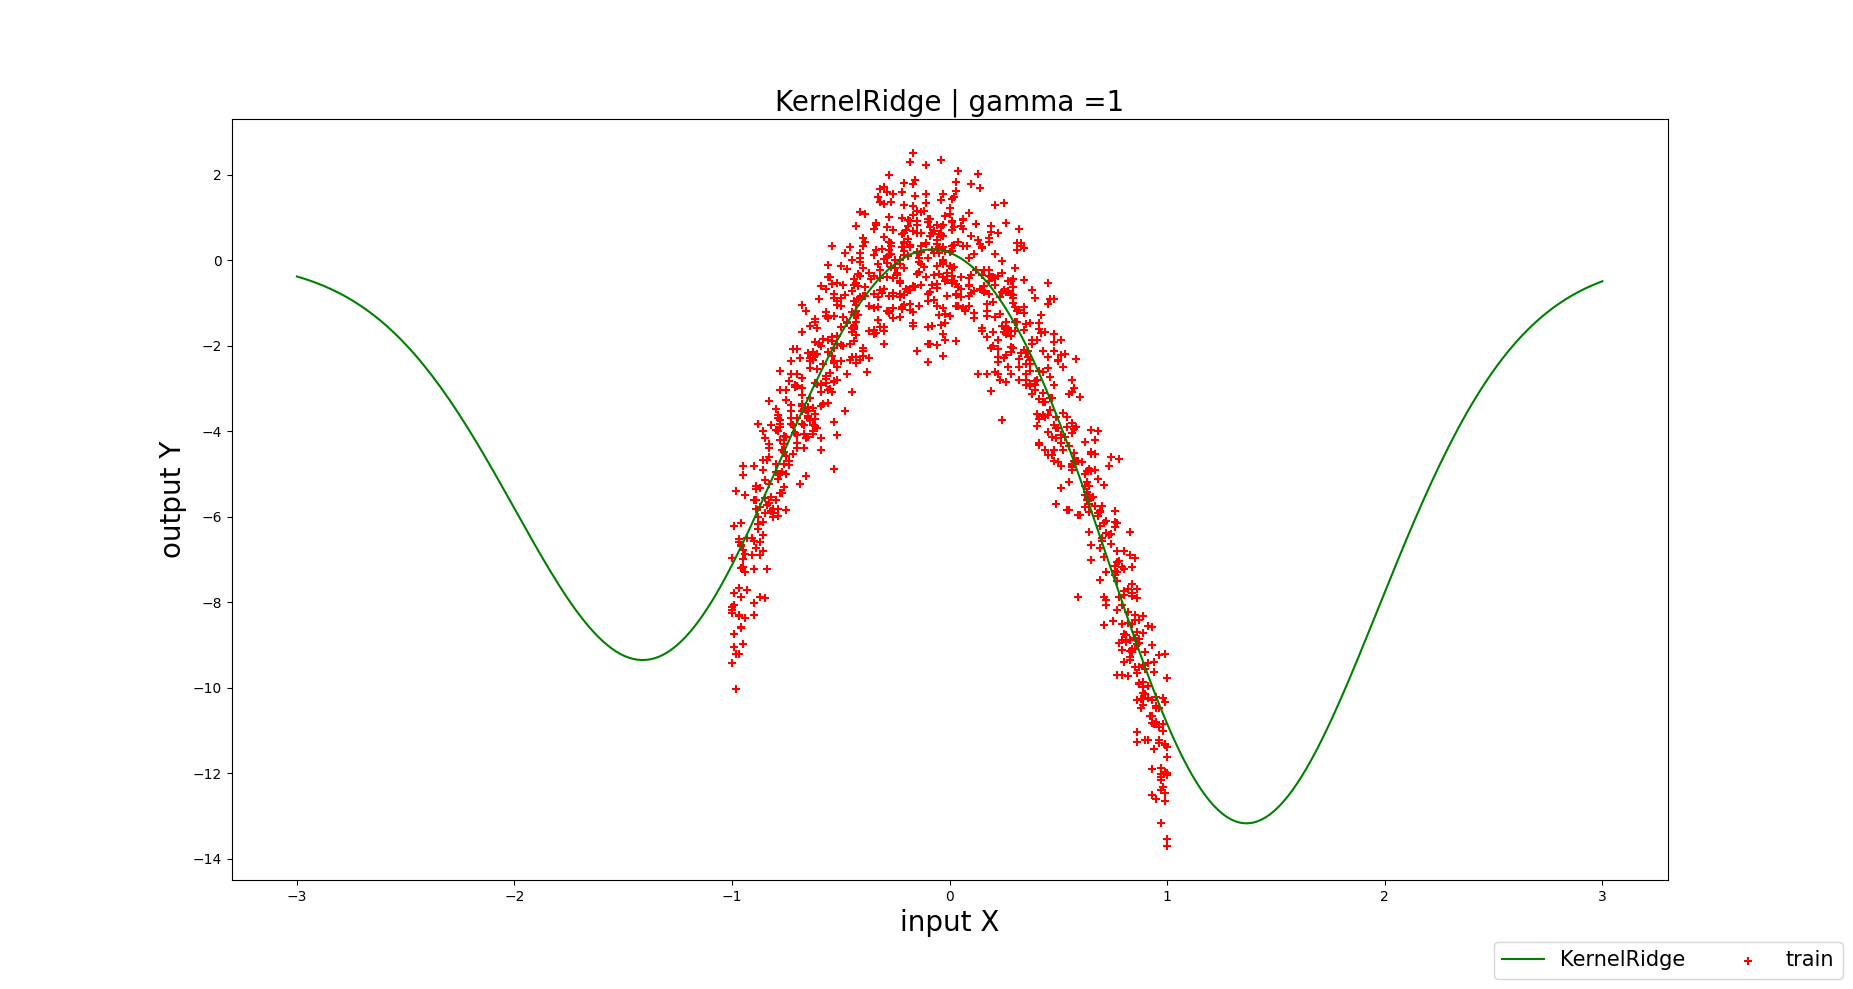
\includegraphics[scale=0.15]{2_kride_gamma_1.png}}   
    \fbox{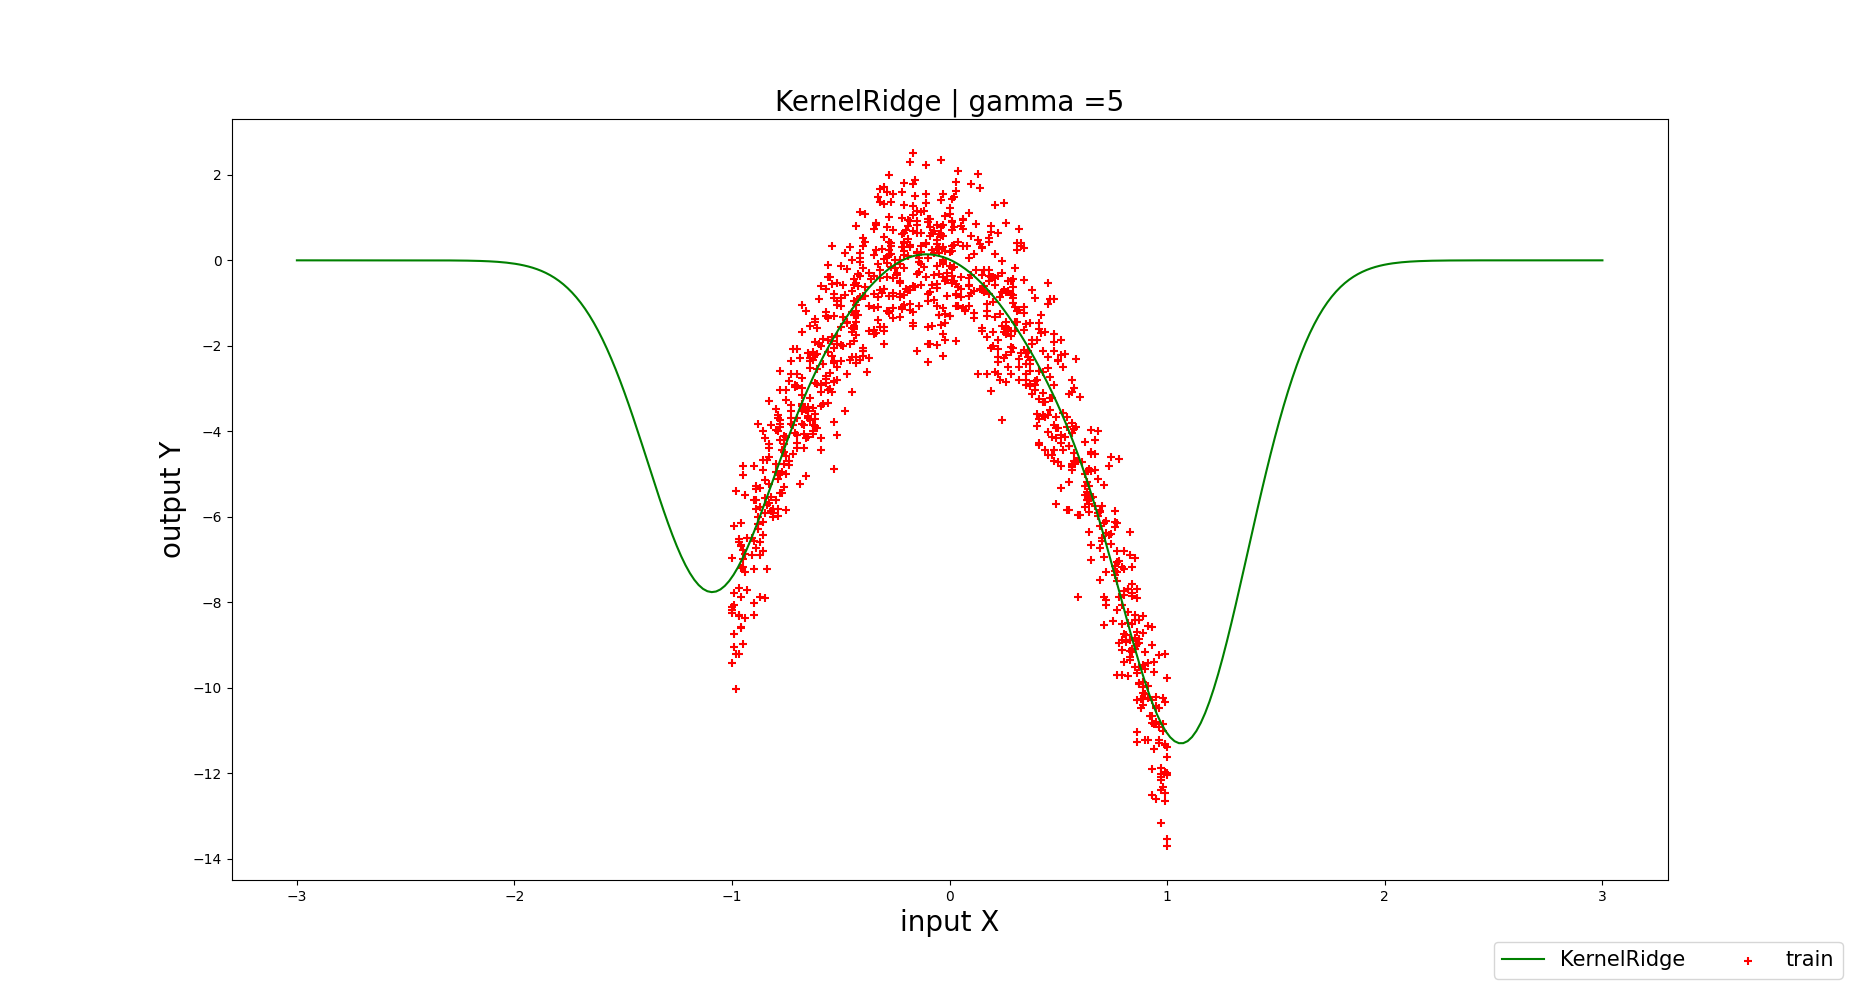
\includegraphics[scale=0.15]{2_kride_gamma_5.png}}
    \fbox{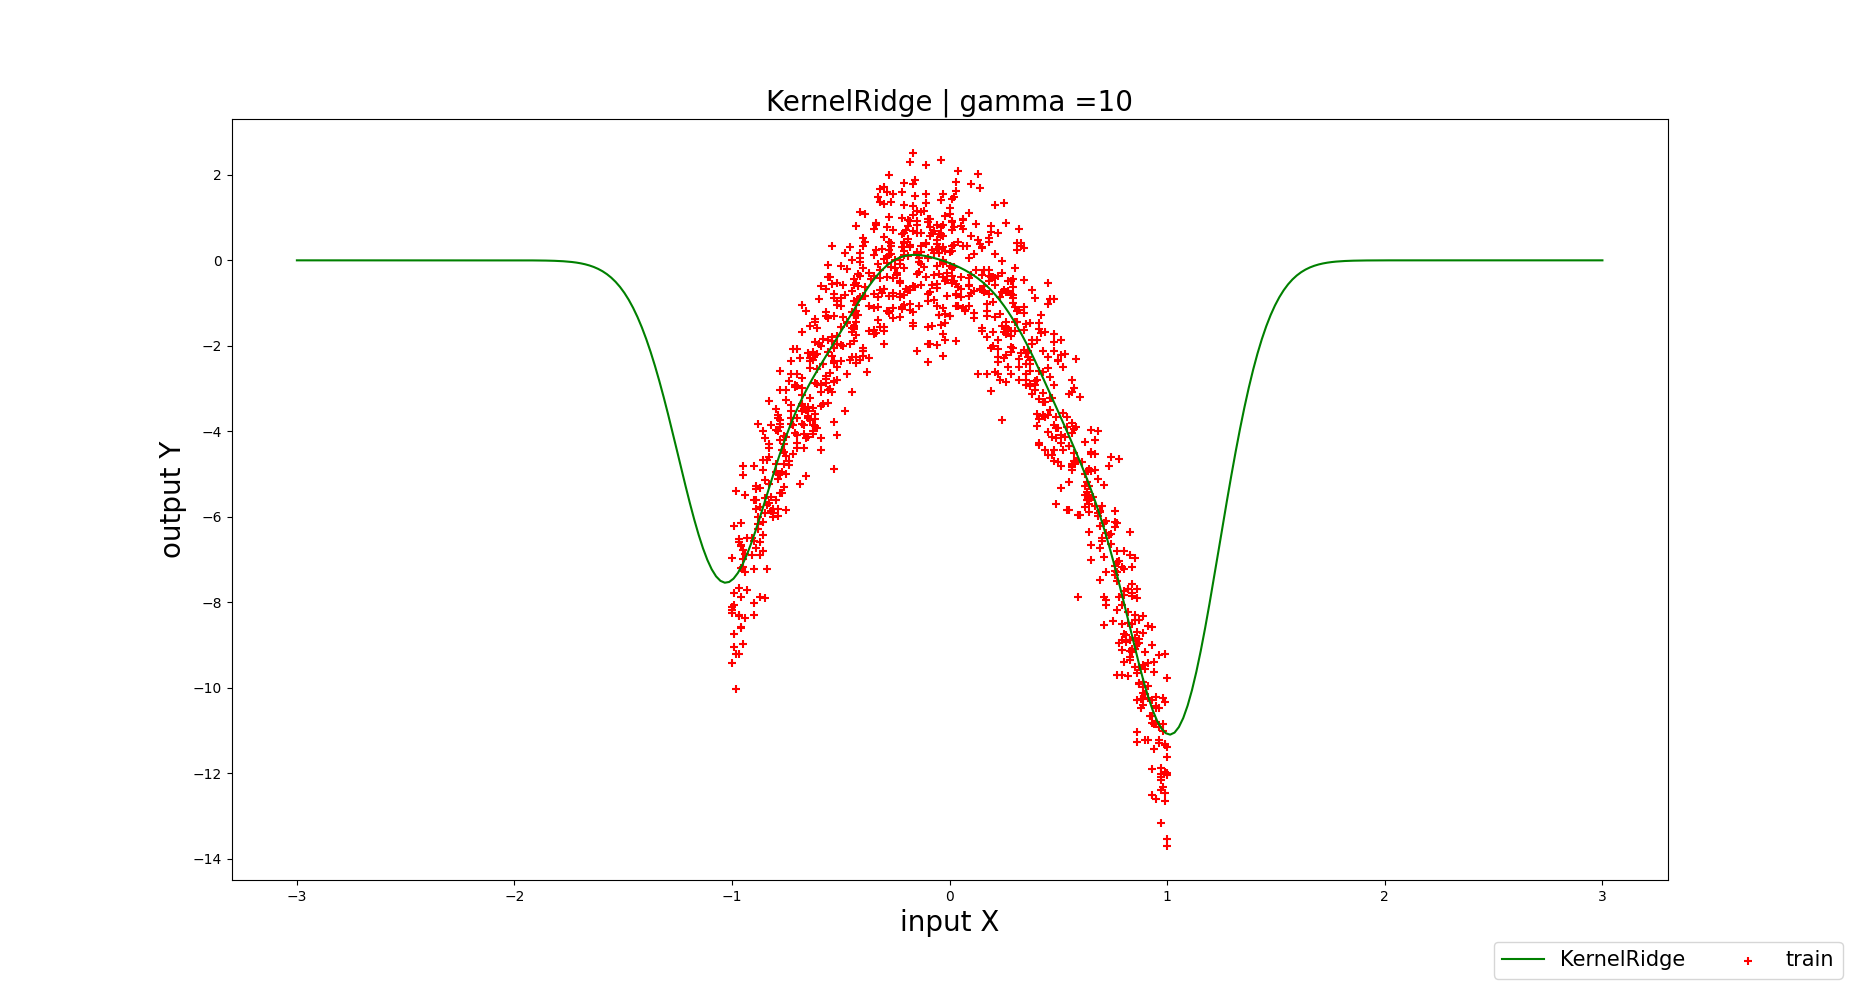
\includegraphics[scale=0.15]{2_kride_gamma_10.png}}
    \fbox{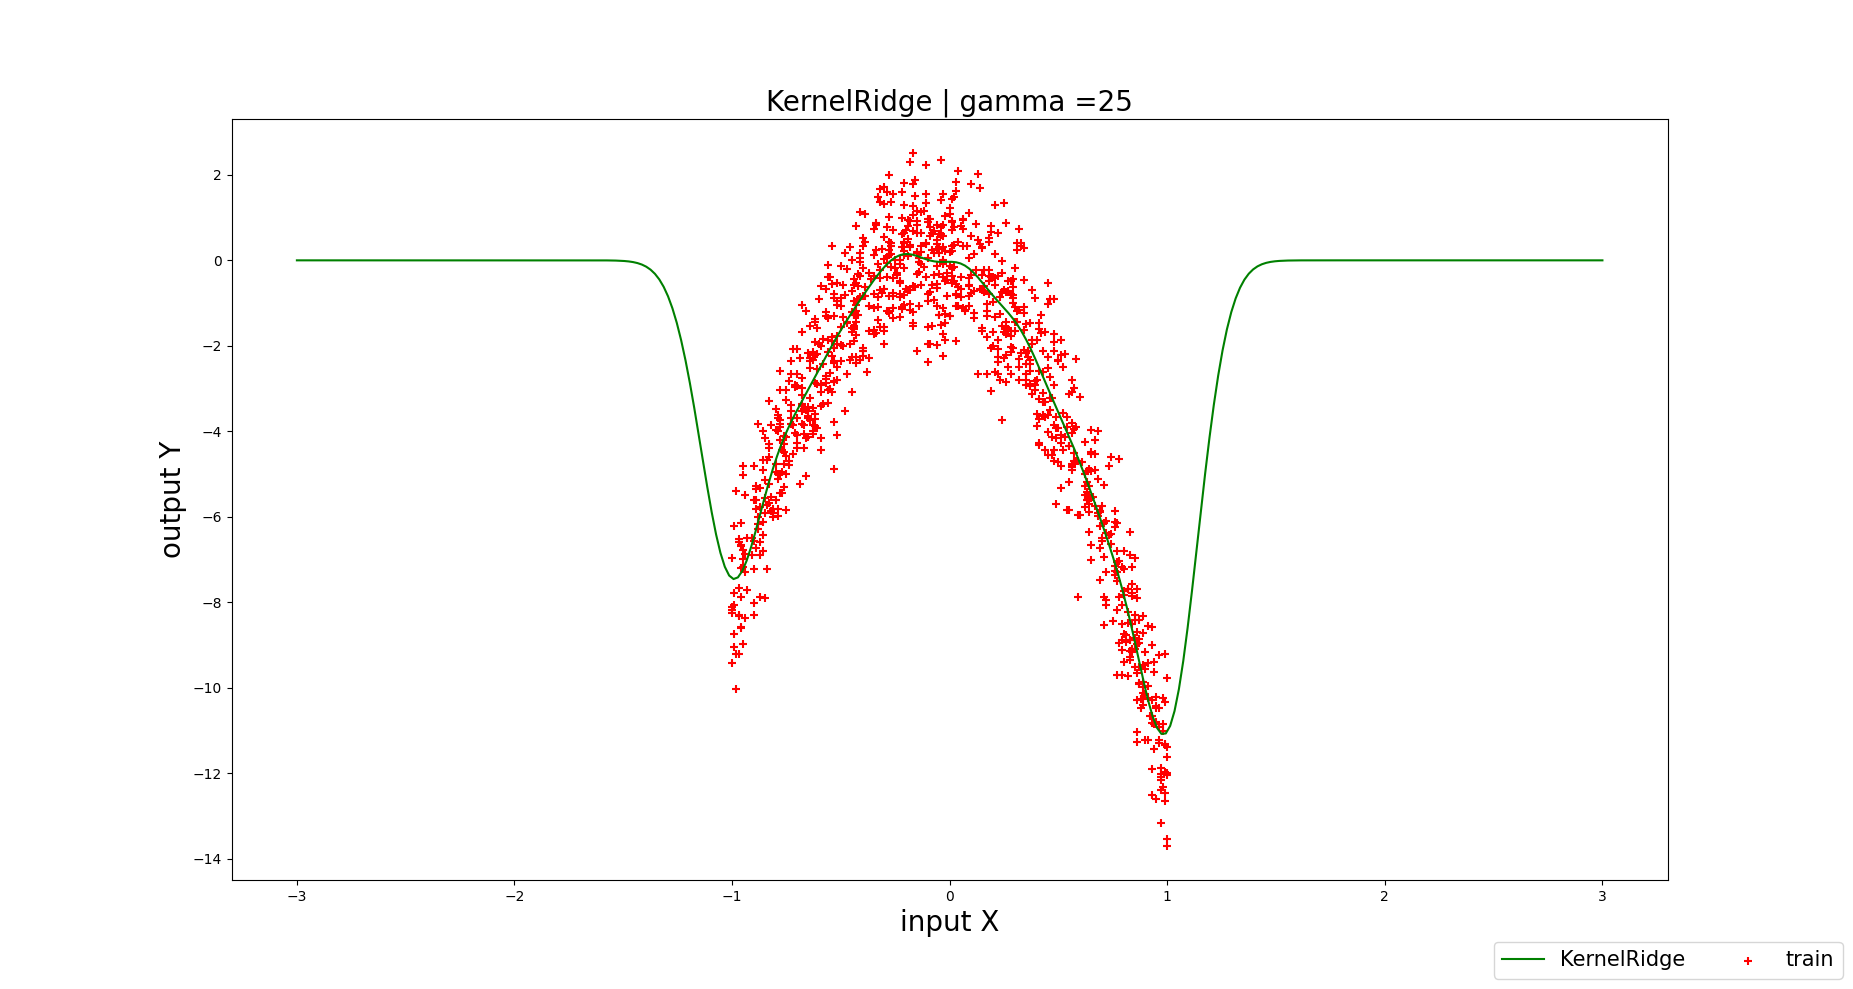
\includegraphics[scale=0.2]{2_kride_gamma_25.png}}
\end{figure}


We notice the same trend as with the kNN model, the more we increase $\gamma$, the more our predictions fit our 
data (and thus its noise), however the main different we notice is in its behavior outside of the training range,
we notice that while the kNN models predicted almost flat negative values, this model moves back up and also becomes
flat, but close to $y = 0$. We could see how depending on our use case we could prefer one or the other model to
make accurate predictions. 

\subsection*{Part c}
Starting with selecting a $\gamma$ value for our kNN model. We use the exact same method for training it as previously
explained, the main difference being that I used a range of values going from 0 to 12, I've found that extending this further
did not provide any value as to making our decision. Then, for each trained model, we keep its score and mean squared error such
as to use them when plotting our cross-validation graph.

\begin{lstlisting}
    scores.append(model.score(Xtrain, ytrain))
    temp.append(mean_squared_error
                (ytrain, model.predict(Xtrain)))
\end{lstlisting}

Then, the actual plotting is quite simple, it only involves using the data from above inside an errorbar from the plotting
library. We obtain the following plot:

\begin{center}
    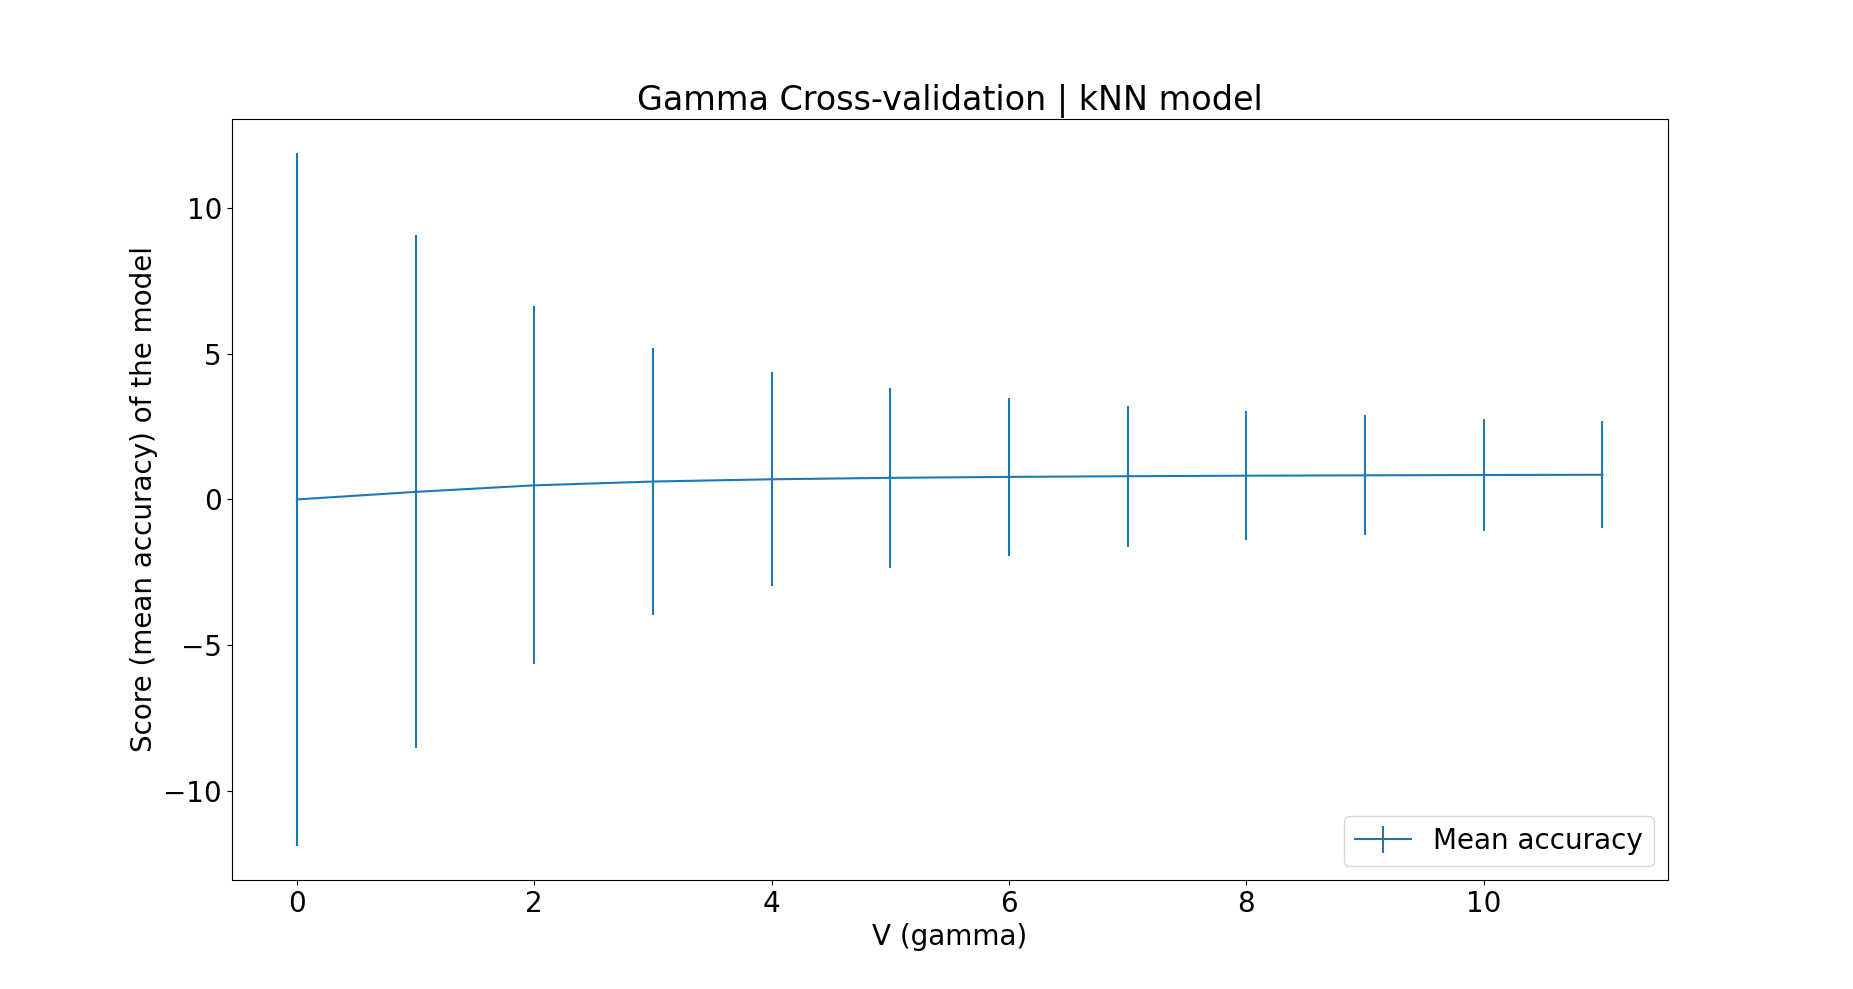
\includegraphics[scale=0.27]{knn_crossval.png}
\end{center}

We notice clear improvements in the mean squared error mostly as we start increasing $\gamma$, it seems
to start settling around $\gamma = 7$. We also notice a bit of an increase in model scores in the range 
$[0, 3]$ however that also setles and remains fairly constant. We will pick a value of $\gamma = 8$ for the
kNN model which seems to be where our values stabilise and give us the best predictions.

Let's now look at the kernalised ridge regression model. We will first do a cross-validation of the $\gamma$ value.
We do so in the exact same manner, except that we use a range of C values this time, I chose to use a range between
$[0, 30]$. We obtain the following cross-validation plot:

\begin{center}
    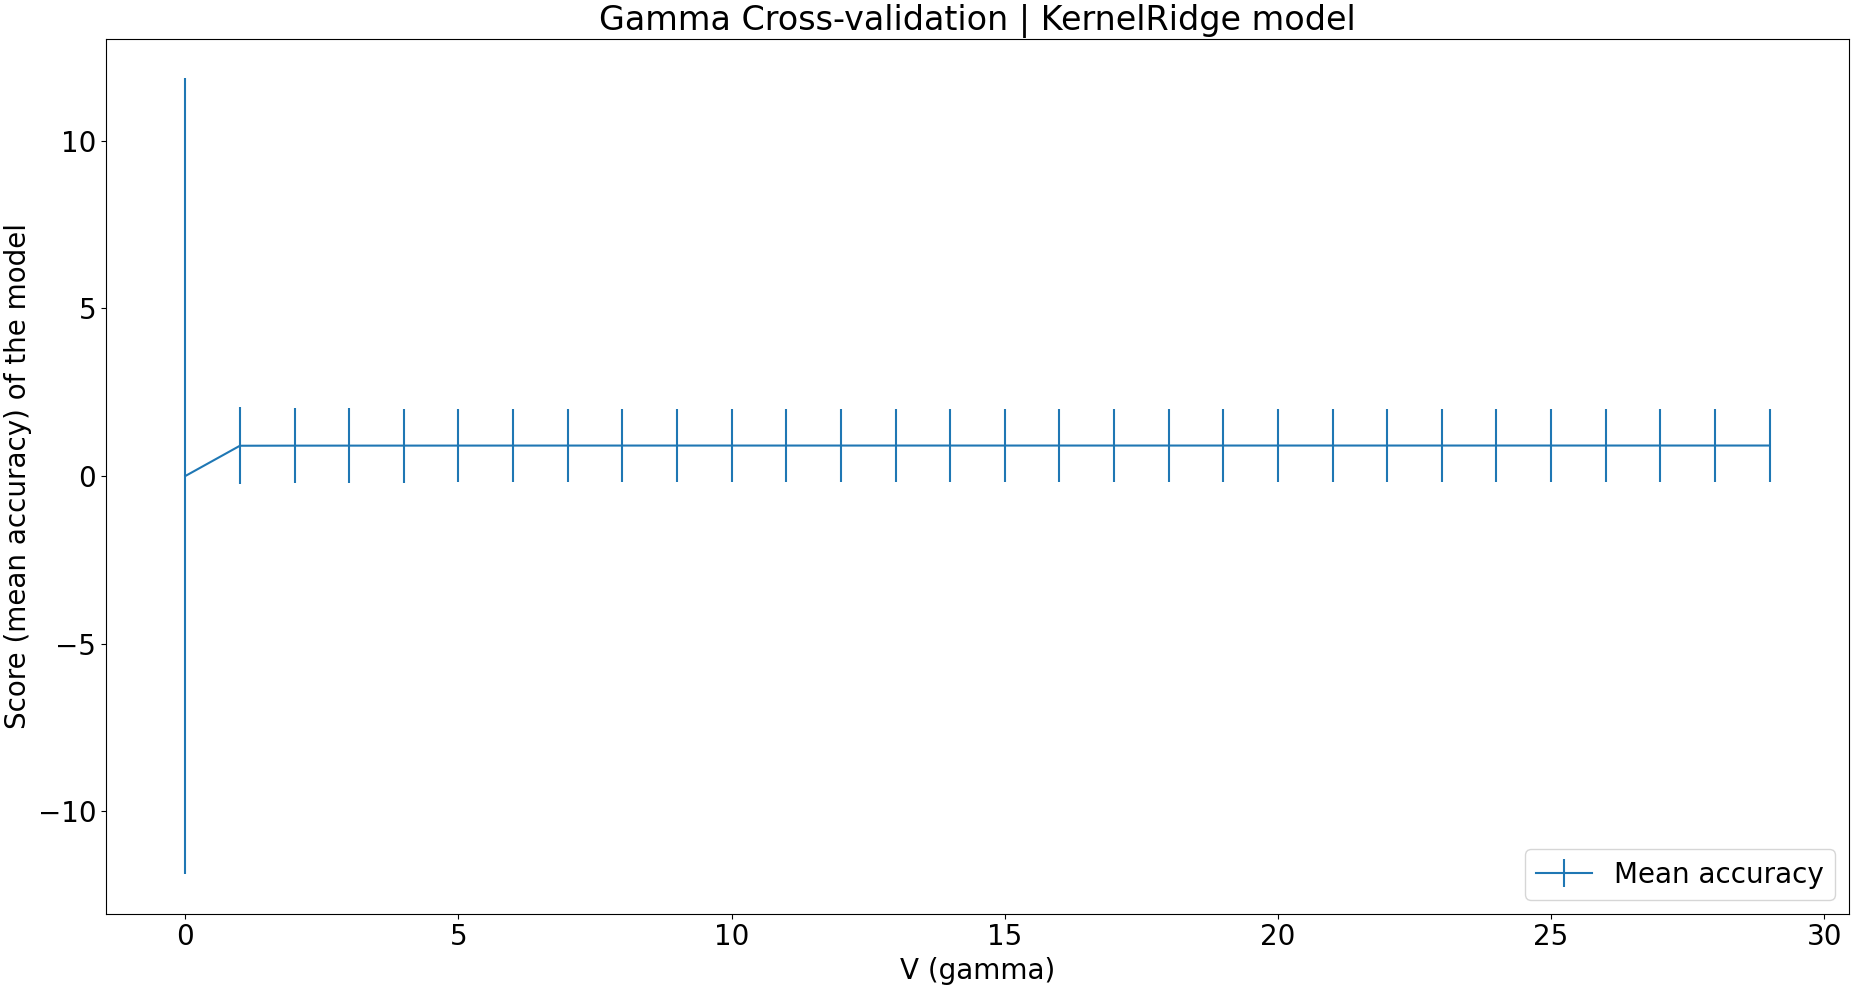
\includegraphics[scale=0.27]{kridge_crossval_gamma.png}
\end{center}

We notice some fluctuations in both score and mean squared error, which seems to stabilise once we reache about
$\gamma = 3$. I've decided to use $\gamma = 4$ for this model as it seemed that increasing it more did not make
a particularity positive impact on predictions.

Finaly, using $\gamma = 4$ for this kernalised ridge model, we can now do a cross-validation of the C value (remember that 
$\alpha = 1 / C$) using the same techniques but varying C this time, I've chosen to use the range of $[0.1, 15]$ with 
a total of 30 evenly values evenly spaced within that range.

\begin{center}
    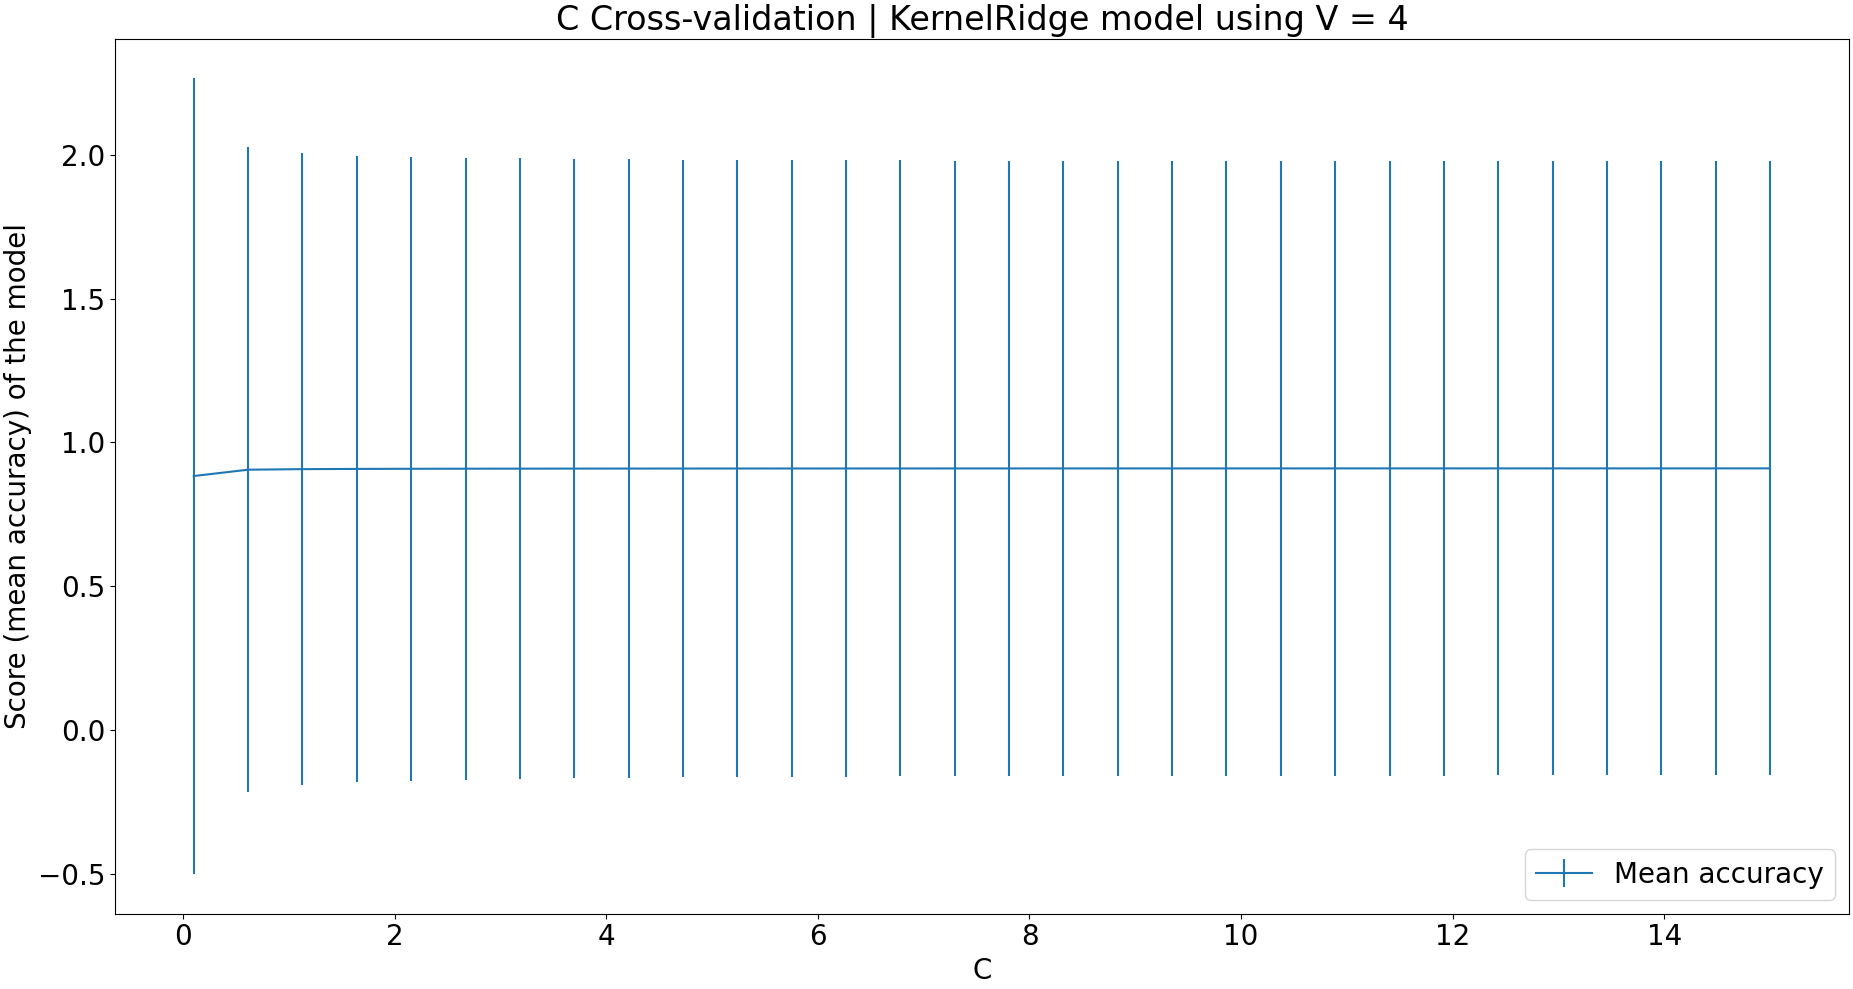
\includegraphics[scale=0.27]{kridge_crossval_c.png}
\end{center}

We notice quite a similar trend, with some fluctuation towards the first part of that plot and stabilisation
after a certain point, here we can use $C = 3$ such as to make our model give the most reliable predictions.

We can now train both models using the values we identified, that is $\gamma = 8$ for the kNN model and 
$\gamma = 4$, $C = 3$ for the kernalised ridge model. The final piece we need is a baseline model such as to
know what to compare our models to, for this I've decided to train a simple DummyRegressor which uses the mean as a
constant prediction. We then obtain the following predictions plot:

\begin{center}
    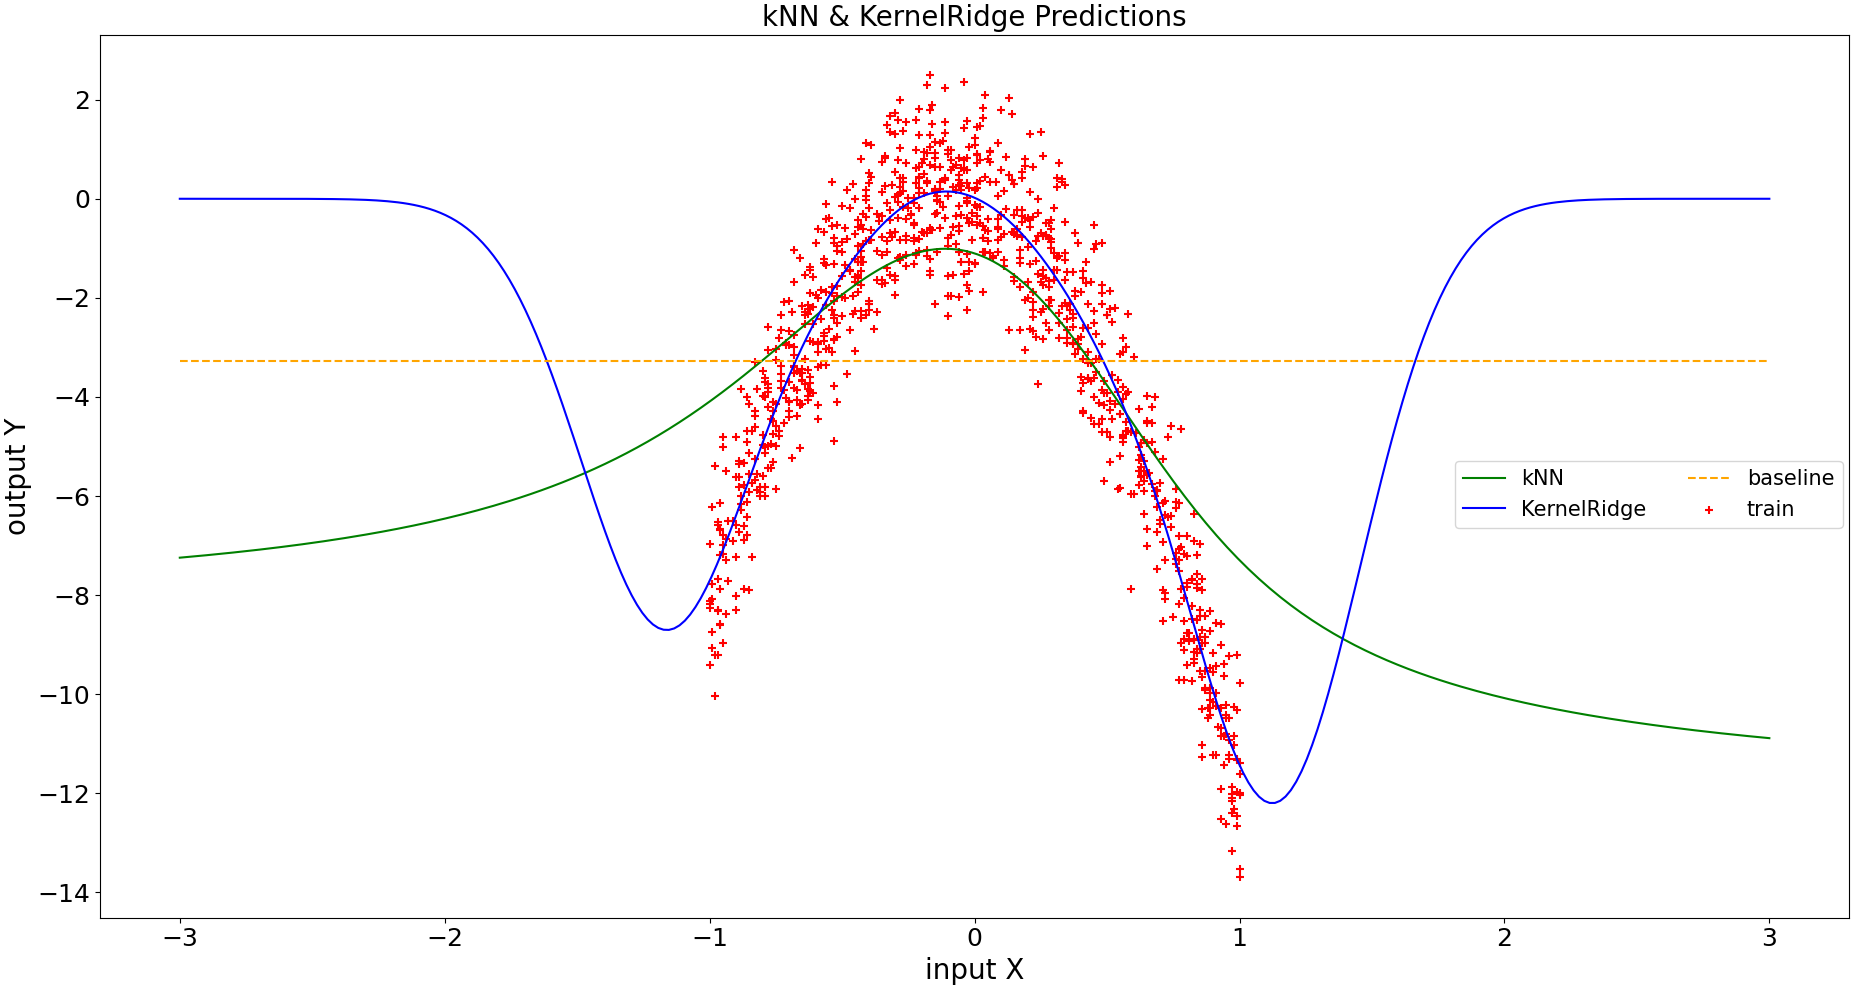
\includegraphics[scale=0.27]{optimised.png}
\end{center}


\section*{Appendix}


\end{document}
